% Lean Agentic AI for Supplier Risk Management and Performance Evaluation — working paper v0.7
% Source of the content: docs/paper/paper.md (v0.7). This file is the typeset, condensed version.
% Build: latexmk -pdf -outdir=build paper.tex  (or: pdflatex paper.tex, run twice)
% Figure 1 and the appendix table are generated by scripts/generate_spider.py,
% Figures 3-6 by scripts/plot_calibration_validation.py.
\documentclass[10pt,twocolumn,a4paper]{article}

\usepackage[T1]{fontenc}
\usepackage[utf8]{inputenc}
\usepackage{textcomp}
\usepackage[margin=2.0cm,columnsep=0.72cm]{geometry}
\usepackage{booktabs}
\usepackage{graphicx}
\usepackage{amsmath}
\usepackage{amssymb}
\usepackage{xcolor}
\usepackage{array}
\usepackage{enumitem}
\usepackage{caption}
\usepackage{titlesec}
\usepackage{ragged2e}
\newcolumntype{P}[1]{>{\RaggedRight\arraybackslash}p{#1}}
\usepackage{tikz}
\usetikzlibrary{arrows.meta,positioning,calc}
\usepackage[hidelinks]{hyperref}

\definecolor{ink}{HTML}{14181B}
\definecolor{ink2}{HTML}{3D474D}
\definecolor{ink3}{HTML}{6E7B82}
\definecolor{rule}{HTML}{C9D1D5}
\definecolor{pblue}{HTML}{2E5A87}
\definecolor{pgreen}{HTML}{3E8F63}
\definecolor{pred}{HTML}{B3372C}
\definecolor{pamber}{HTML}{B57C15}

\captionsetup{font=small,labelfont=bf,labelsep=period,justification=justified}
\captionsetup[table]{skip=4pt}
\setlist{nosep,leftmargin=1.2em}
\titlespacing*{\section}{0pt}{2.0ex plus .3ex}{0.9ex}
\titlespacing*{\subsection}{0pt}{1.4ex plus .2ex}{0.6ex}
\renewcommand{\arraystretch}{1.12}
% float placement: without these, late figures are deferred past the
% bibliography and land on near-empty pages
\renewcommand{\topfraction}{0.92}
\renewcommand{\bottomfraction}{0.70}
\renewcommand{\textfraction}{0.06}
\renewcommand{\floatpagefraction}{0.70}
\setcounter{topnumber}{3}
\setcounter{totalnumber}{5}
\raggedbottom

\newcommand{\dimhead}[1]{\textbf{#1}}
\newcommand{\ev}[1]{{\footnotesize\textsc{#1}}}
\newcommand{\code}[1]{{\small\texttt{#1}}}
\newcommand{\synth}{\textit{Synthetic data.}}
\newcommand{\ptsq}{points\textsuperscript{2}}

\title{\vspace{-1.4em}\Large\bfseries Lean Agentic AI for Supplier Risk Management\\
and Performance Evaluation\\[0.35em]
\large\mdseries Turning spreadsheet scorecards into transparent, expert-calibrated
multi-agent systems: a benchmark of four approaches and an open-source demonstrator}
\author{Csaba Bakay}
\date{Working paper, draft v0.7 \textperiodcentered{} October 2026}

\begin{document}
\maketitle

\begin{abstract}
\noindent
Procurement organisations evaluate their suppliers twice: \emph{supplier risk
management} asks how exposed the company is if a supplier fails, \emph{supplier
performance evaluation} how well the supplier delivers. In practice the two are often
split: a commercial risk platform is licensed for risk, while performance evaluation stays
in spreadsheets, so that one supplier is judged on two inconsistent bases. Spreadsheet
scorecards are transparent but cannot learn, scale or keep an audit trail; risk platforms
bring data coverage and workflows at a cost, with limited control over how scores are
formed, and, according to their public documentation, do not cover performance
evaluation. Open-source agent projects show how such systems could be built, but their
focus is the agent architecture rather than the scoring method. Across all
of them, the weights that turn criteria into a score are set once and never checked
against the judgement of the people who know the suppliers.
This paper makes three contributions. It proposes fifteen success factors, including
the integration of risk management and performance evaluation, corrected in documented
reviews. It profiles four approaches on them without aggregating them: spreadsheet
practice, two commercial platforms, five open-source repositories and the approach
proposed here; the profiles are the author's qualitative expert assessment from public
information and code review (October 2026), not a measurement. And it presents
\emph{Lean Agentic AI} with an open-source demonstrator whose main difference from pure
risk platforms, as far as their public documentation shows, is the integration of both
views: risk management and performance evaluation on one criteria catalogue, each with its
own weights, classes and actions. The demonstrator is an agentic workflow in a narrow
sense --- deterministic, specialised agents over a shared state in a LangGraph graph,
including a calibration agent, routed by a rule-based supervisor and paused for human
review; scoring, calibration, recommendations and routing use no language model, and one
optional, explicitly triggered and so far unevaluated component uses one only to interpret
final results, without changing scores, classes or weights --- with deterministic, material-group-specific scoring, weights calibrated
against category managers' expert labels by constrained least squares, versioned
weights, and concrete actions per factor.
All experiments use synthetic data only, with labels from a hidden weighting plus noise
or from constructed expert policies; no real expert labels were used and no field
validation was performed. On these synthetic portfolios, calibration reduced the cross-validated error between score and label from 37.8 to
20.6~\ptsq{}, close to the irreducible label noise of 18.1, and moved the weights about
half-way towards the hidden weighting. Regularisation was essential with few labels.
When the simulated experts judge non-additively, apply knock-outs, are uniformly
stricter or disagree, calibration degrades in characteristic ways, each pointing to a
design response other than calibration. The validation also exposed an acceptance rule
that let harmful calibrations through; its replacement, a cross-validated rule that
requires the improvement to exceed its own uncertainty, cut harmful acceptances from up
to 50\,\% of runs to at most 4\,\%.
The paper states what this does not establish: the labels are synthetic, the benchmark
ratings are the author's own judgement (including of the author's own demonstrator),
predictive validity against real disruptions is untested, and the demonstrator provides only
partial external signal coverage, without live monitoring. No ranking of approaches is
derived at any point.
\end{abstract}

{\small\tableofcontents}
\vspace{0.6em}

% ═══════════════════════════════════════════════════════════════════════
\section{Introduction}
\label{sec:intro}

Supplier risk evaluation has moved from an annual formality to a recurring management
task. Disruptions in logistics, energy and geopolitics have made supply concentration
visible, and supply-chain risk management research has long described identifying,
assessing, treating and monitoring risk as one connected process
\cite{tang2006,ho2015,fan2018}. This paper is concerned with the \emph{assessment}
stage. Due-diligence regulation expects documented risk analysis along the supply chain,
and procurement teams are asked to show not only \emph{which} suppliers are risky, but
\emph{why}, and what was done about it.

A common response is to extend the supplier scorecard: the criteria sheet gains columns
for financial stability, supply-chain exposure and ESG, and a weighted average turns
them into a score and a traffic light. Where budgets allow, a commercial platform
supplies alerts and external data. Both responses leave a gap. The spreadsheet keeps the
method in the procurement team's hands but does not keep a record: weights drift
between versions, and no one can say afterwards why a supplier was rated as it was. The
platform brings data coverage and workflows, but the method by which its score is formed
is, depending on the vendor, partly or largely outside the customer's view. Open-source
agent projects offer modern architecture but rarely a scoring method that would stand
up in an audit.

A second gap is rarely discussed. Risk platforms address \emph{supplier risk
management}; \emph{supplier performance evaluation} --- delivery reliability, quality,
price, responsiveness, graded A, B or C --- is a separate, established process. A common
pattern in practice is that a company licenses a risk platform and still runs its
supplier evaluation in spreadsheets. The same supplier is then judged in two systems,
with different criteria, scales and update cycles, and nobody sees both pictures side by
side. A supplier can deliver excellently and still be a critical dependency; that is
exactly the case the split hides.

One problem cuts across all three options and is rarely named: \textbf{the weights are
not validated.} A scorecard may weight business impact at fourteen per cent and ESG at
twelve. Those numbers usually come from a workshop, a template or a vendor default, and
are seldom checked against the holistic judgement of the category managers who know the
suppliers best.

This paper takes a deliberately lean route. It does not propose a new risk taxonomy or
data source. It starts from the scorecard practice that already exists --- for risk and
for performance --- and asks what it would take to evaluate both on one consistent basis
and to make that practice \emph{transparent} (method and weights documented),
\emph{reproducible} (every number recomputable), \emph{governed} (human approval where
judgement is required) and \emph{able to learn} (weights aligned with expert judgement)
--- at the cost profile of open-source software. The argument proceeds in two steps: a
benchmark of four approaches on fifteen success factors (Figure~\ref{fig:profile}), read
factor by factor without weighting, total or ranking, as a qualitative expert assessment
by the author rather than a measurement; and an open-source demonstrator, so that each
claimed property can be inspected in code, tests and documentation rather than asserted.
The demonstrator and all experiments run on synthetic data; no real expert labels or field
data were used. This has a cost, discussed in
Section~\ref{sec:limitations}, and a benefit: because the labels were generated from a
known hidden weighting, it can be checked whether calibration recovers it.

\paragraph{Terminology.} ``Agentic'' denotes an \emph{orchestrated multi-agent
workflow}: the agents (data collection, scoring, calibration, recommendation, human
review) are deterministic Python functions acting as nodes of a LangGraph state graph, a
rule-based supervisor routes between them, and the workflow pauses for human approval.
Scoring, calibration, recommendations and routing use no language model. The only
exception is an optional \emph{Supplier Review Agent} that, on explicit request, asks a
language model to interpret one supplier's final results and cannot change scores, classes
or weights (Section~\ref{sec:aireview}); document extraction and an LLM-based supervisor
are planned extensions only. The term does not imply autonomous, LLM-driven decision
making.

\begin{figure*}[t]
  \centering
  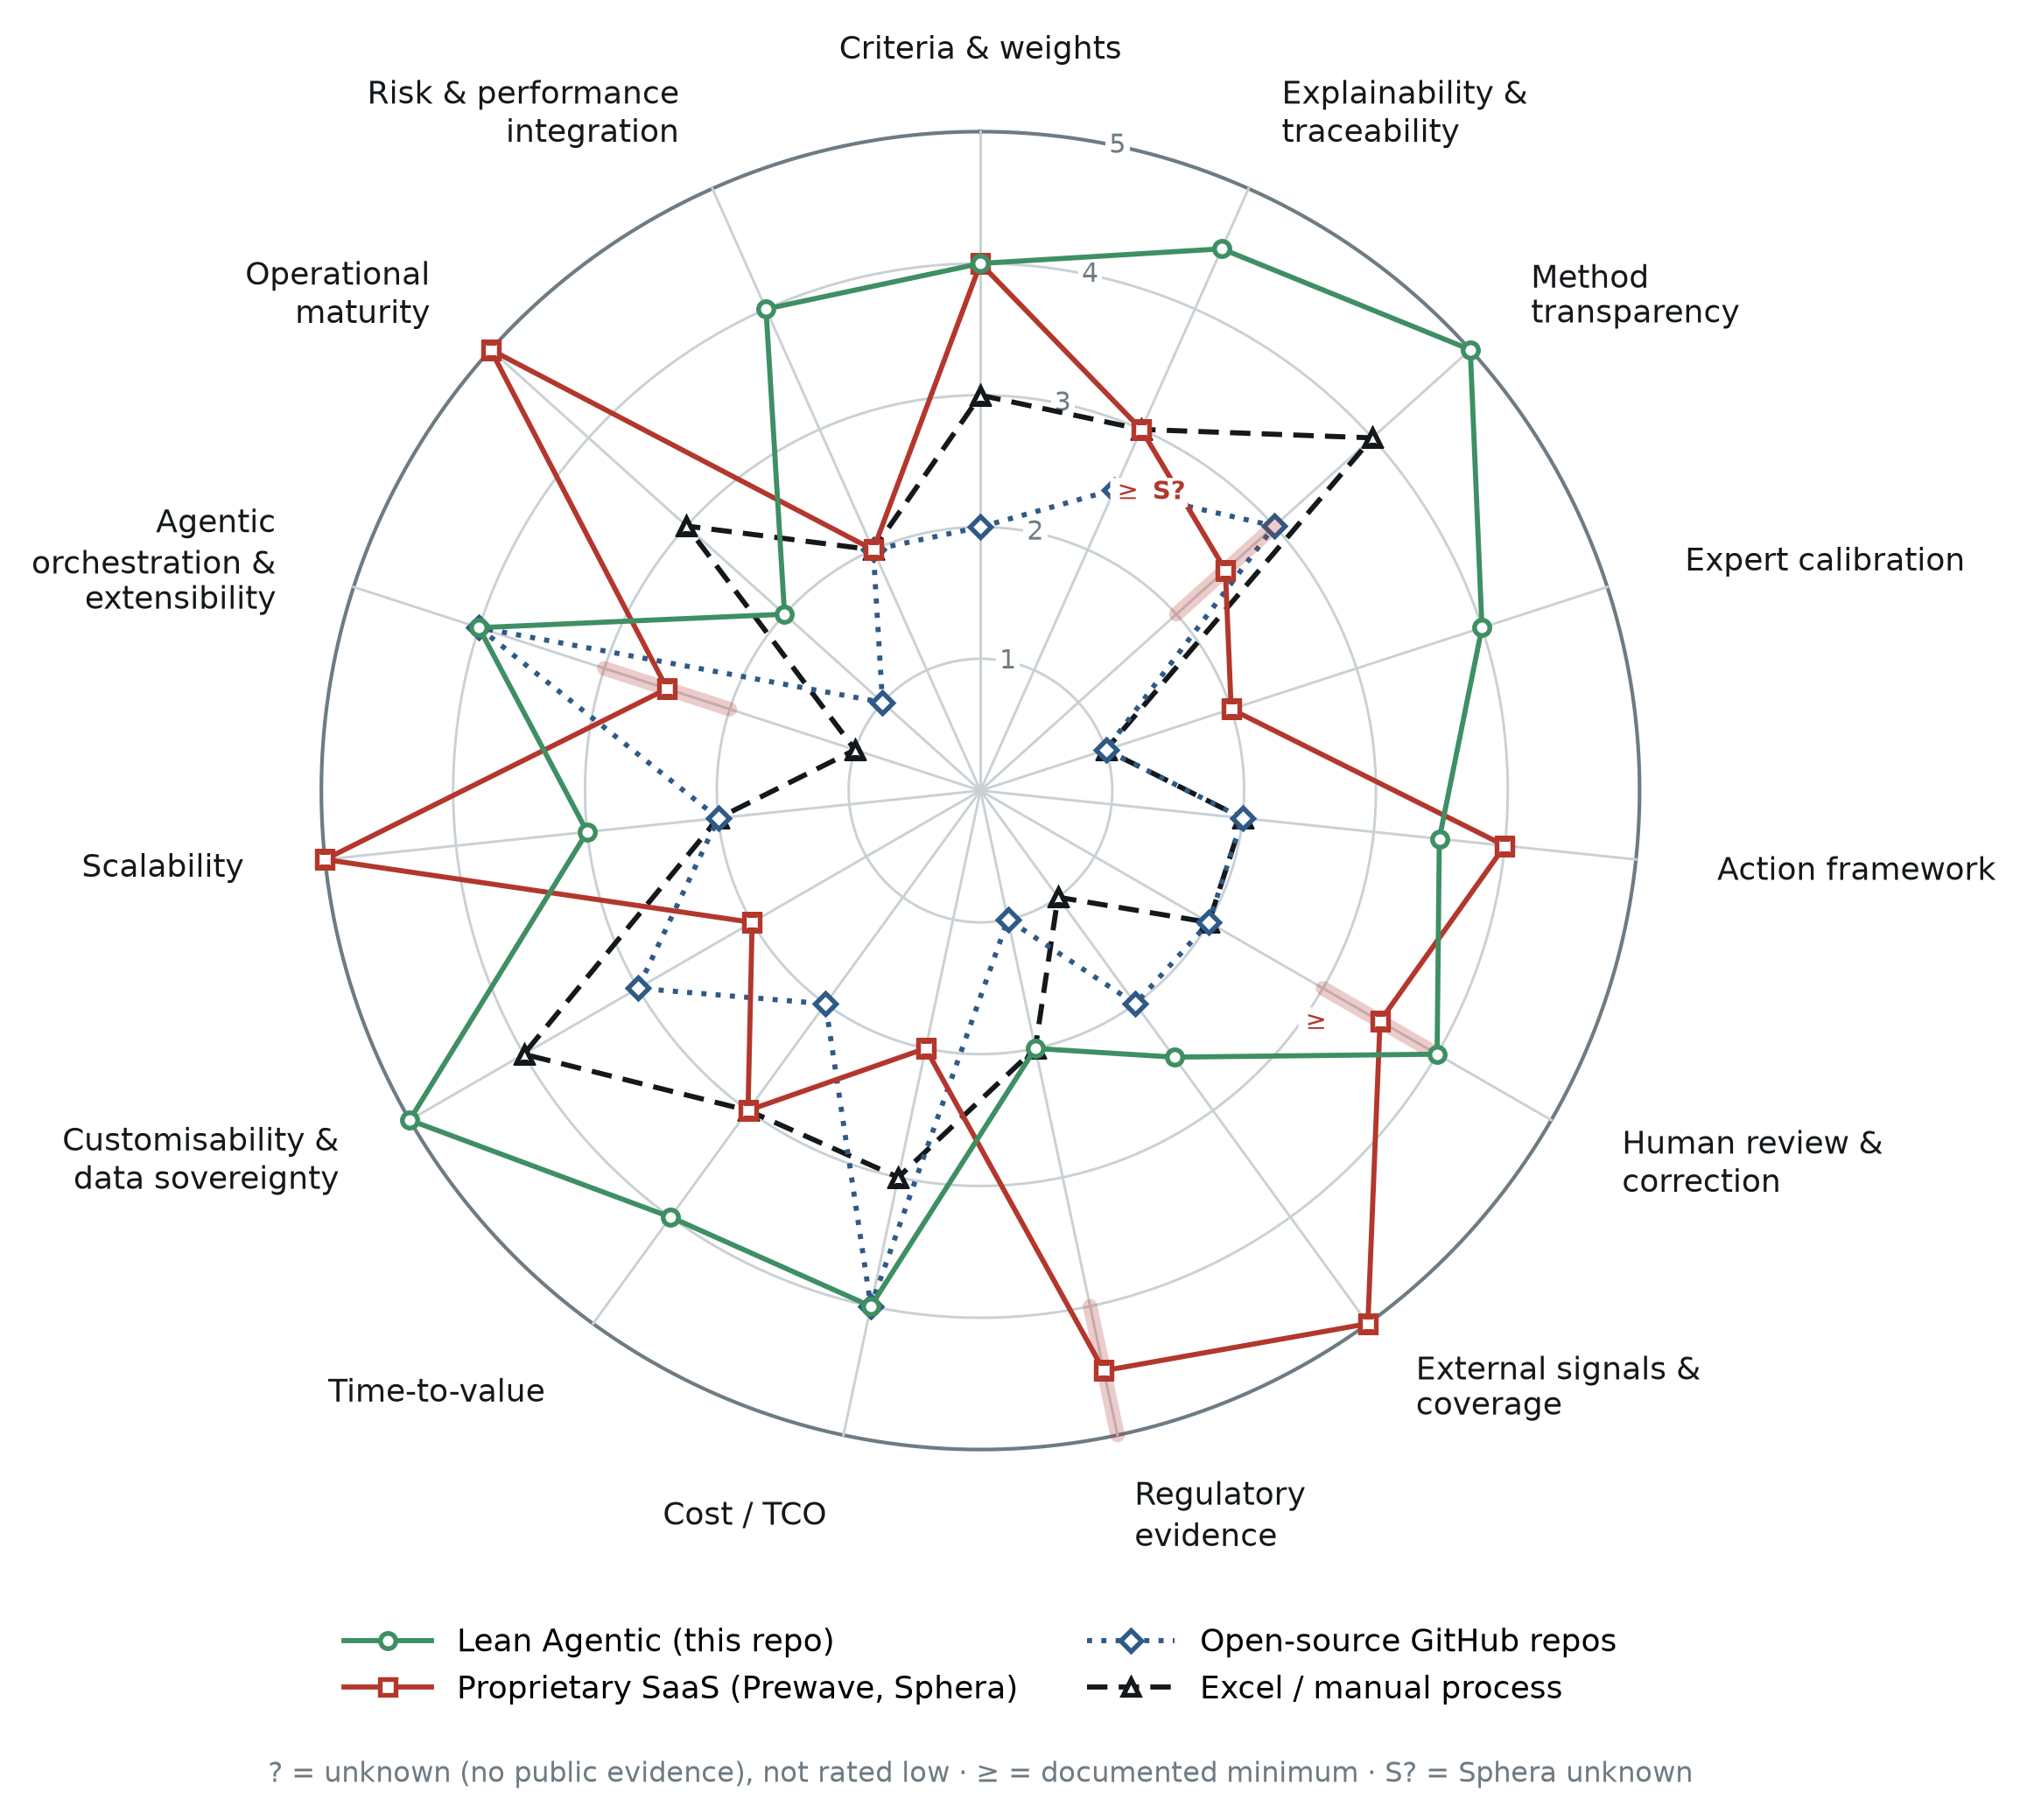
\includegraphics[width=0.74\textwidth]{figures/fig01_benchmark_profile.png}
  \caption{Four approaches to supplier risk management and performance evaluation profiled
  on fifteen success factors (model v0.4), on a five-level scale; half points mark a
  profile between two levels. Proprietary SaaS is plotted as the mean of
  Prewave and Sphera; shaded bars mark where the two differ. Rationale and confidence for
  every value: Table~\ref{tab:matrix} and \code{research/comparison-matrix.md}.
  \textbf{Illustrative, qualitative assessment by the author based on public information
  and code review, October 2026; expert judgement, not an empirical measurement.} The author
  also built one of the rated approaches. The factors stay separate: no weighting is applied, no total is formed and no
  ranking is derived.}
  \label{fig:profile}
\end{figure*}

\paragraph{Contributions.}
\begin{enumerate}
  \item \textbf{Fifteen success factors} for supplier risk management and performance
  evaluation, including their integration, each with a definition and the evidence by
  which it can be assessed, together with the documented reviews that produced the
  current version (Section~\ref{sec:factors}).
  \item \textbf{A profile benchmark} of four approaches. Every value comes from one
  machine-readable source with a rationale and a confidence mark; the two commercial
  examples are rated separately (Section~\ref{sec:benchmark}).
  \item \textbf{The Lean Agentic approach}, a synthesis of scorecard practice, platform
  expectations and open agentic architecture. Its positioning rests on two features: the
  integration of risk management and performance evaluation, and calibration against
  expert labels inside an agentic workflow (Section~\ref{sec:approach}).
  \item \textbf{An open-source demonstrator}: a LangGraph workflow of deterministic
  agents with deterministic scoring, material-group weights, constrained least-squares calibration, a
  graph-interrupt review step, versioned weights, two views (performance evaluation and
  risk management), an action framework, an assessment history and an optional,
  experimental LLM-based review of final results that changes no number
  (Section~\ref{sec:architecture}), examined in five experiments on synthetic data
  (Section~\ref{sec:demo}).
  \item \textbf{An explicit statement of what is not established}, and of the work that
  would close each gap (Sections~\ref{sec:limitations}--\ref{sec:future}).
\end{enumerate}

% ═══════════════════════════════════════════════════════════════════════
\section{Background and related work}
\label{sec:background}

\subsection{Supplier risk assessment in practice}
Weighted multi-criteria aggregation is the dominant instrument for evaluating suppliers.
Reviews of the supplier-selection literature catalogue the analytic hierarchy process,
outranking, data envelopment analysis, mathematical programming and fuzzy or hybrid
approaches \cite{ho2010,chai2013}; most share one structure of criteria, weights and an
aggregation rule. Case studies show formal and informal supply-risk assessment processes
in use, frequently in scoring form \cite{zsidisin2004}. A typical supplier-risk scorecard
has a \emph{severity} component (how replaceable is the supplier, how badly would a
failure hurt) and \emph{likelihood} components for financial stability, supply-chain
exposure and ESG or compliance, rated on an ordinal 1--5 scale, weighted and aggregated
into a score and a class. The method is not in question here; how it is run is:
definitions are informal, weights are set once, results are not reproducible after the
file has changed, and consequences are free text, if they are written at all.

\subsection{Commercial supply-chain risk platforms}
Two platforms serve as named examples, assessed \textbf{on public information only}
(vendor websites, help-centre articles, press releases, as of October 2026); nothing here
is a product test. \textbf{Prewave} combines continuous media and trade-data monitoring
with supplier assessments and due-diligence modules. Unusually, it publishes the
composition of its supplier score: a peer component (country, industry, commodity) at
30\,\%, alerts at 40\,\%, assessments at 20\,\% and external data at 10\,\%, aggregated
non-linearly. Event types and weights can be adjusted in customer-specific
``perspectives''; source weighting and signal classification are not disclosed.
\textbf{Sphera Supply Chain Risk Management} offers portfolio risk views, multi-tier
mapping, early warnings, response playbooks and a documented bundle for the German
supply-chain due-diligence act. Its scores are described as ``AI-scoring'' tied to
business impact; no public description of the method or of customer-adjustable weights
was found.

Both use AI: Prewave for signal processing and with connectors for external AI agents,
Sphera with fine-tuned generative models for supplier risk summaries and marketed
``agentic AI'' capabilities. Three observations matter. ``Platform'' is not one
methodological profile: on transparency the two examples differ by a full scale point,
which is why they are rated separately. \textbf{Neither documents calibration against
the customer's own expert judgement}: weight adjustment exists, but as configuration,
not as a fitted and reported procedure. And \textbf{both are risk platforms}: neither
documents a supplier performance evaluation with its own criteria and grades, nor a
customer-inspectable multi-agent workflow --- specialised agents over a shared state, a
calibration agent, a review pause in the workflow graph --- in public sources. This
describes public documentation as of October 2026, not the products themselves.

\subsection{Open-source agentic supply-chain projects}
Five public repositories were reviewed at source-code level. They converge on one
architecture --- specialised agents sharing a typed state, coordinated by a graph or a
supervisor --- and diverge sharply on scoring. One contains no scoring at all; two
compute deterministic, hard-coded weighted scores, one of them deliberately overwriting
numbers produced by the language model; two leave the risk judgement to a language
model, and in one a published example contains arithmetic errors in the weighted
totals, which illustrates the risk of letting a language model generate numbers. Two carry no licence, one a copyleft licence, and none ships an automated test
suite. The repositories are most useful here as \textbf{architectural blueprints}; their
focus differs from the scoring-method focus of this paper. This work reuses ideas from
them, but no code.

\subsection{Calibrating weights against expert judgement}
Two practices both go by the name of ``setting weights'': \emph{eliciting} them directly
by asking how important each criterion is, and \emph{inferring} them from holistic
judgements of how risky each supplier is overall.

\textbf{Direct elicitation is method-dependent.} Different procedures (swing, SMART,
trade-off, pairwise comparison) produce systematically different weights for the same
problem \cite{borcherding1991,poyhonen2001}, and weight judgements are subject to range
insensitivity and splitting biases \cite{weber1993}. Weights agreed in a workshop are one
plausible answer among several, not a measurement.

\textbf{Inferring weights has two traditions.} \emph{Judgement analysis and policy
capturing}, rooted in Brunswik's lens model \cite{hammond1955}, regresses holistic
judgements on cues to recover the weights a judge implicitly uses
\cite{aimansmith2002,karren2002}. Linear models reproduce such judgements well
\cite{karelaia2008}, and a model of a judge can outperform the judge by applying the
policy consistently \cite{goldberg1970}. The tradition also cautions that ``improper''
weights, for example equal weights, often perform about as well as fitted ones
\cite{dawes1979}: gains from fitting should be modest, and fitted weights should not
stray far from sensible priors. \emph{Preference disaggregation} infers an additive value
model from holistic evaluations, in the UTA family by linear programming on rankings
\cite{uta1982,uta2001}. The calibration here belongs to the same family but fits
\emph{cardinal} scores by least squares, constrains the weights to a simplex with a lower
bound, and shrinks them towards a prior. With few judgements and many weights, a fit
adapts to noise; ridge regularisation trades a small bias for a large reduction in
variance \cite{hoerl1970}, and shrinking towards a prior instead of zero is a direct
generalisation \cite{hastie2009}. Directly elicited weights thus serve as the prior, and
holistic labels adjust them under constraints.

\subsection{Language models and determinism}
For risk scores, language models are the wrong default. A score that changes when the
same input is presented twice cannot be audited; outputs can vary across identical
requests even at temperature zero, as shown for code generation \cite{ouyang2025}. A
score that cannot be recomputed by hand cannot be challenged. The more mature reviewed
designs compute numbers in code and reserve the language model for language. This paper
adopts that division strictly: its one language-model component
(Section~\ref{sec:aireview}) only interprets numbers that code has already computed.

% ═══════════════════════════════════════════════════════════════════════
\section{Success factors}
\label{sec:factors}

An approach is easier to assess when the properties that matter are named before any
approach is rated. Table~\ref{tab:factors} proposes fifteen such \emph{success
factors}, each with the observable evidence that would let someone else check a rating.
They form a \textbf{flat list}: not arranged in a hierarchy, not weighted and not
combined into a total. An approach is read as a \textbf{profile}; one that is strong on
twelve factors and absent on one is a different proposition from one that is uniformly
adequate, and a single figure would treat the two alike.

\begin{table*}[t]
  \caption{Success factors for supplier risk management and performance evaluation (model
  v0.4). The factors are
  read separately; no weighting, total or ranking is derived from them.}
  \label{tab:factors}
  \small
  \begin{tabular}{@{}P{0.02\textwidth}P{0.20\textwidth}P{0.345\textwidth}P{0.345\textwidth}@{}}
    \toprule
    & \dimhead{Success factor} & \dimhead{What it means} & \dimhead{Assessable by} \\
    \midrule
    1 & Structured criteria \& weights & Explicit criteria, scales and weights combining measurable indicators and structured expert assessment & Criteria with definition and scale; explicit weights; both input types with provenance \\
    2 & Traceability \& reproducibility & Every result can be reconstructed and recomputed from documented inputs & Per-result record; change history; recomputation; tests \\
    3 & Methodological transparency & The method is documented and checkable \emph{before} use & Published formula, weights, sources, rules \\
    4 & Expert calibration & Parameters are systematically fitted to expert judgement, with approval & Procedure; fit metric; logged old and new parameters; approval \\
    5 & Action framework & Results map to defined actions, review cycles and owners & Actions per class and driver; tracking to closure \\
    6 & Human-in-the-loop \& governance & Defined review and approval points, recorded decisions, roles & Approval steps; recorded overrides; roles \\
    7 & External signals \& coverage & Current external data and breadth of supplier coverage & Sources, update frequency, languages, tier-N \\
    8 & Regulatory evidence & Support for due-diligence documentation duties & Regulation-specific workflows and reports \\
    9 & Cost / TCO & Total cost of use, including recurring internal effort, and access barriers & Licence model, prices, implementation effort, manual effort per cycle \\
    10 & Time-to-value & Time and effort to the first usable result & Time to first portfolio assessment \\
    11 & Customisability \& data sovereignty & The organisation can change method and implementation, including material-group configuration, and controls its data & Configurable without vendor; per-group criteria, weights or thresholds; licence; data location \\
    12 & Scalability & Works as suppliers, users, groups and update frequency grow & Suppliers handled; marginal effort; automation \\
    13 & Agentic orchestration \& extensibility & Work is orchestrated as an explicit workflow of specialised agents; new capabilities can be added without rebuilding the core & Specialised agents over a shared, inspectable state; review pauses in the workflow; extension points; APIs \\
    14 & Operational maturity \& support & Production readiness & Support, service levels, security, release process \\
    15 & Risk \& performance integration & Supplier risk and supplier performance are evaluated on one consistent basis, each with its own logic & Shared criteria and data; separate weights, classes and actions per view; both results per supplier \\
    \bottomrule
  \end{tabular}
\end{table*}

\subsection{How the factor model was derived, and corrected}
The first version (v0.1) was drawn up from the requirements of the proposed approach. A
critical review identified four problems, documented because they bear on how far the
benchmark can be trusted. \emph{Means presented as ends}: ``open source'' and
``multi-agent orchestration'' named the means one had chosen, which makes the comparison
circular; both were reframed as outcomes (customisability and data sovereignty;
extensibility). \emph{Home-field bias}: v0.1 contained only one factor on which
platforms are clearly stronger; \emph{regulatory evidence} and \emph{operational
maturity} were added. \emph{Overlaps}: structured criteria and objective/subjective
inputs, and audit trail and determinism, were merged; transparency (understanding the
method before use) was kept apart from traceability (reconstructing a result
afterwards). \emph{Validity}: no factor asks whether a score \emph{predicts}
disruptions. No reviewed approach reports predictive validity publicly, so the factor
cannot be rated today; it is left off the radar and treated as an open question.

A second review (v0.3) followed informal practitioner feedback, not a structured survey
(numbers in this paragraph refer to v0.3). It added factor 16,
\emph{integration of risk management and performance evaluation}, because the common
split between a risk platform and spreadsheet-based evaluation was not captured by any
factor. It sharpened factor 14 to \emph{agentic orchestration and extensibility}, because
``uses AI'' and ``is an agentic workflow'' were indistinguishable; the factor stays an
outcome --- explicit, inspectable, extensible orchestration --- but its evidence now names
agents with shared state and review pauses. And it widened factor 10 to the total cost of
ownership, including recurring manual effort. Factor 16 is one on which the proposed
approach is strong, and factor 14 moves partly back towards an architecture property
that v0.2 had reframed; both are disclosed as such. The four factors on which the
commercial examples are clearly ahead (8, 9, 13 and 15) are unchanged.

A third review (v0.4) reduces the model to fifteen factors. Material-group adaptation
(old 5) becomes evidence under customisability and data sovereignty (old 12, now 11):
per-commodity configuration is a specific case of changing the method. Its separate axis
double-counted that capability. Integration remains unchanged (old 16, now 15); old 1--4
retain their numbers and old 6--16 become 5--15. All retained scores, confidence marks and
per-vendor values stay unchanged. The customisability rationales now include group
configuration and its limits; the removed scores are retired, not averaged. The retained
customer-control ratings are Excel 4/M, SaaS 2/M, open repos 3/H and Lean Agentic 5/H.
For open repos, visible code supports modification, but neither supplies group adaptation
nor removes licence constraints. Platform strengths retain their scores (now 7, 8, 12, 14).

The remaining boundaries separate structure from control, configuration from fitted
calibration, method transparency from historical reconstruction, actions from approval,
lifecycle cost from adoption time and capacity, customer control from workflow extension,
and generic audit records from regulatory documentation. Governance concerns decision
rights; operations concerns reliable service, infrastructure security and support. Joint
risk/performance evaluation remains distinct from a structured single-view model. This is
conceptual separation, not proven statistical independence: a $4\times15$ rating matrix
has rank at most four, or three after centring. Independent validation is still needed;
the full overlap review is in \code{research/success-factors.md}.

% ═══════════════════════════════════════════════════════════════════════
\section{Benchmark: four approaches profiled}
\label{sec:benchmark}

\subsection{Method}
Four approaches are rated on a five-point scale (1 weak or absent, 3 adequate, 5 very
strong); a half point marks a profile clearly between two levels. The ratings are the
author's qualitative expert judgement from public information, source-code review and
practitioner experience; they are not measurements, and no product was tested. Each rating carries a rationale and a confidence mark: \textsc{h} verified from
code or primary documentation, \textsc{m} plausible and partly documented, \textsc{l}
assumption. All ratings live in one machine-readable file from which
Figure~\ref{fig:profile} and Table~\ref{tab:matrix} are generated; a consistency check
fails if the published table no longer matches the source. The evidence differs by
approach, and this is disclosed (Table~\ref{tab:condensed}): spreadsheet practice is a
stereotype based on the author's practitioner experience; Prewave and Sphera are rated separately on
public information; the five repositories by source-code review; and the demonstrator
\emph{as implemented}, not its roadmap.

\begin{table}[t]
  \caption{Condensed benchmark (author's assessment, not a measurement): strongest (4--5)
  and weakest (1--2) factors per approach; factors rated 1 are in bold. Full matrix:
  Appendix, Table~\ref{tab:matrix}.}
  \label{tab:condensed}
  \small
  \begin{tabular}{@{}P{0.20\columnwidth}P{0.36\columnwidth}P{0.32\columnwidth}@{}}
    \toprule
    \dimhead{Approach} & \dimhead{Strongest} & \dimhead{Weakest} \\
    \midrule
    Excel / manual & Transparency; customisability & \textbf{Calibration; external signals; agentic orchestration}; traceability; actions; human-in-the-loop; regulatory evidence; scalability; risk \& performance integration \\
    SaaS (Prewave, Sphera) & External signals; scalability; operational maturity; regulatory evidence; criteria \& weights; action framework; human-in-the-loop & Cost; customisability; calibration; risk \& performance integration \\
    Open-source repos & Cost; agentic orchestration & \textbf{Calibration; regulatory evidence; operational maturity}; most other factors \\
    Lean Agentic & Transparency; customisability; risk \& performance integration; calibration; agentic orchestration; traceability; criteria \& weights; cost; time-to-value & Regulatory evidence; operational maturity \\
    \bottomrule
  \end{tabular}
\end{table}

\subsection{Reading the profiles}
\textbf{Spreadsheet practice is strong where simplicity helps}: it keeps formulas
visible and can be changed by the team itself. It costs no licence but a great deal of
recurring manual work, and a governed scorecard takes weeks to build. It is weak wherever
a system property is needed --- an audit trail, learning, external data, orchestration ---
and risk and performance usually live in separate files. Real practices vary widely, and
a well-governed workbook can do better than the stereotype.
\textbf{The commercial platforms are strongest on data, scale and operations}: external
signals, regulatory evidence, scalability and operational maturity, with well-developed
workflows. They are weaker on cost, self-determined customisation, recomputability by the
customer (a design consequence of continuous monitoring rather than a flaw) and, for one
of the two, transparency; their spread is largest exactly there. They are risk
platforms: performance evaluation is not part of their documented scope, and their AI is
not exposed as an inspectable multi-agent workflow.
\textbf{The open-source repositories are blueprints}: free to license but demo-grade,
with agent architectures as their main asset; they are rated rudimentary on most
methodological factors, which reflects a different focus rather than a failed method.
\textbf{The Lean Agentic demonstrator is strongest where the method itself matters}:
transparency, traceability, expert calibration and customisability (including
material-group configuration) --- and on the two factors that set it apart from pure risk platforms,
the integration of risk management and performance evaluation and agentic orchestration
(both 4, against 2 and 2.5 for the platforms). It is close to the platforms on actions
and human review (3.5 against 4): the action framework and the graph-based review pause
exist, but tracking to closure and roles do not. It is better than spreadsheets on cost of
ownership and time-to-value, because scoring, actions and reports run automatically from
a template. On external signals it reaches about half of the strongest platform (2.5
against 5): the provider interface reads open data and system exports and records their
origin, while live APIs are still placeholders and there is no continuous monitoring. The
architecture allows further providers, and an external-signal agent is a natural extension;
this upside is not rated. The approach remains weak on regulatory evidence and operational
maturity. These dips define what the approach is not.

\subsection{Complementary, not ranked}
The profiles do not order the approaches. Lean Agentic does not replace the data
coverage of a platform. The realistic reading is \textbf{complementary}: a platform or
open data serves as the \emph{signal source}, and a transparent, calibrated model owned
by procurement turns signals and internal knowledge into classes and actions
(Section~\ref{sec:hybrid}).

\subsection{Threats to validity}
\emph{Author bias}: the factors and all ratings come from a single rater, the author, who
also built one of the rated approaches and thus rates their own work. The v0.2 correction, rating the demonstrator as implemented, and a rationale
and confidence mark for every value reduce the bias but do not remove it. The v0.3
review works in the other direction: it added a factor on which the proposed approach is
strong and re-rated five factors after practitioner feedback, all of them in its favour
(action framework, human-in-the-loop, time-to-value and external signals upwards; cost of
spreadsheets and repositories downwards). The re-ratings are documented with their
rationale and rate the implementation, not the roadmap; expected upside, for example in
signal processing, is named but not rated. An independent re-rating is future work. \emph{Public information only} for the platforms: hands-on
evaluation could move several ratings. \emph{Date dependency}: all platform ratings refer
to October 2026. \emph{Ordinal scale}: differences of one point are not measured
distances.

% ═══════════════════════════════════════════════════════════════════════
\section{The Lean Agentic approach}
\label{sec:approach}

\subsection{Definition and synthesis}
\emph{Lean Agentic AI} is defined here as an approach that starts from the evaluation
practice an organisation already has, uses open agentic workflows as blueprints, and
builds a tailored, transparent, low-cost system on top of that practice rather than
replacing it. ``Lean'' means building only what adds value, reusing open blueprints, and
keeping the method with the team that is accountable for it.

\paragraph{Positioning: one basis for risk and performance.} The approach is not a
further risk platform. Its main difference from pure risk platforms such as Prewave and
Sphera, as far as their public documentation shows (October 2026), is that it evaluates \emph{supplier risk management} and \emph{supplier
performance evaluation} on one consistent basis: one criteria catalogue, one data sheet,
one engine, and two views with their own logic (Section~\ref{sec:views}). This closes the
gap described in the introduction, where a risk platform and a spreadsheet evaluation
judge the same supplier separately. It does not replace the platform's signals; it can
consume them as indicators (Section~\ref{sec:hybrid}). The second pillar is that the
method is run by an agentic workflow whose agents --- including a calibration agent ---
share an inspectable state and stop for human approval inside the graph. The agents that
score, calibrate, recommend and route are deterministic code without a language model; an
optional review agent uses one only to interpret final results
(Section~\ref{sec:aireview}).

The approach inherits from each tradition in Section~\ref{sec:background}. \emph{From
scorecard practice} it takes the domain logic: named criteria, 1--5 ratings, weighted
dimensions including a severity component (availability of alternatives, change
complexity, business consequence) and class-based actions. Procurement keeps its method
and vocabulary; the method becomes explicit, versioned and testable. \emph{From
commercial platforms} it takes the expectations placed on a professional system: review
and approval steps, an audit trail, integration of objective indicators with expert
assessment, and an action framework. External signal feeds are not implemented; they
are intended to come from open data or a platform, through the provider interface of
Section~\ref{sec:actions}. \emph{From open-source agent projects} it takes the
architecture --- a supervisor coordinating specialised agents over a typed state --- and
the lesson that numbers are computed in code.

\subsection{Distinguishing features}
Eight features distinguish the approach; the first three carry its positioning.
\textbf{(1) Integration of risk management and performance evaluation.} Each criterion
is defined once, with its meaning and rating source, and shared where both views need it
(for example credit risk or compliance status). Each view has its own dimensions,
weights, classes, escalation rules, actions, expert labels and approvals; risk is classed
low to critical, performance graded A to C. A supplier is seen in both views from the same
data, and calibrating one view never changes the other. Neither commercial example
documents performance evaluation as part of its platform.
\textbf{(2) Calibration against expert judgement}, the central methodological
contribution. Each
labelled supplier receives a holistic risk score from 0 to 100 on the model's own scale,
and the weights are chosen to minimise the squared error between model score and label,
subject to a minimum weight per factor and weights summing to one. A ridge term pulls the
solution towards the configured defaults, which protects small samples from overfitting
and keeps criteria the methodology considers relevant from being switched off silently.
The anchor is always the configured default, never a previous calibration, so repeated
calibration on the same labels cannot drift; this problem was found by a test. Weights
are accepted only if the \emph{cross-validated} error falls clearly
(Sections~\ref{sec:acceptance} and~\ref{sec:e5}) and are then applied or proposed for
approval, as configured (the bundled risk template proposes by default), and old and new weights, errors and
class agreement are reported. None of the reviewed repositories, and neither commercial
example in its public documentation (as of October 2026), offers this.
\textbf{(3) Agentic orchestration.} The method runs as a graph of specialised agents ---
data collection, scoring, calibration, recommendation, human review --- over one typed,
inspectable state, coordinated by a rule-based supervisor with bounded loops; each of
these agents is a deterministic Python function without a language model, and only the
optional review agent calls one, to interpret final results. The calibration agent
proposes weights; the review is a pause in the graph that resumes with a recorded
decision. The commercial examples use AI for signal processing, summaries and, in one
case, marketed ``agentic'' capabilities, but neither documents such a workflow publicly.
The agents orchestrate; they do not decide (Section~\ref{sec:discussion}).
\textbf{(4) Weights as versioned objects}: default, material-group and calibrated
weights are interchangeable, never hard-coded, and every applied set is written as a new
version with timestamp, approver, model version and metrics.
\textbf{(5) Material-group awareness}: weights can be set and calibrated per commodity,
and each supplier is scored with the most specific set available.
\textbf{(6) Human-in-the-loop as a real pause}: when data is insufficient or weights are
proposed, the workflow stops until a reviewer approves weights, sets a class with a
comment, or defers; manual classes survive re-scoring.
\textbf{(7) Deterministic scoring}: every number is produced by pure, tested functions
and can be recomputed by hand; language models are kept out of the numbers, and their one
implemented role is an optional interpretation of final results.
\textbf{(8) Governance by construction}: escalation rules set class floors that no
average can hide, a completeness check flags results resting on too little data, the
audit trail is append-only, and every feedback loop is bounded.

\subsection{What the approach is not}
It is not a data provider (it monitors no news, disasters or tier-N networks, and ships
no real external data), not a regulatory compliance product, not production-hardened (no
roles, no central run store), and not empirically validated (calibration has been shown
on synthetic labels only). The claim is narrower: the \emph{method layer} of supplier
risk evaluation can be made transparent, reproducible, governed and able to learn at low
cost --- a layer that platforms leave partly opaque and spreadsheets leave ungoverned.

% ═══════════════════════════════════════════════════════════════════════
\section{Architecture of the demonstrator}
\label{sec:architecture}

\subsection{Workflow}
The demonstrator is a LangGraph state graph in hub-and-spoke form
(Figure~\ref{fig:workflow}). A rule-based \textbf{supervisor} inspects the shared state
and routes to one of five workers, plus an optional sixth: \emph{data collection} loads the suppliers in scope
(optionally one material group) with indicators and expert labels, and lets optional
data providers fill missing indicators; \emph{scoring} rates factors, aggregates,
normalises, classifies, applies escalation rules and checks completeness;
\emph{calibration} is optional; \emph{recommendation} maps classes, elevated dimensions
and factor levels to actions, owners and review cycles; \emph{human review} pauses the
run; the optional \emph{AI review} runs only on explicit request
(Section~\ref{sec:aireview}). Every worker returns to the supervisor, and the calibration
loop and review loop each run at most once per run. The supervisor and the five core
workers are deterministic Python code without a language model; the AI review node is the
only place that calls one. The routing rules fit in one function, which is also
the single, so far unused, extension point for a planned language-model-based supervisor.

\begin{figure}[t]
  \centering
  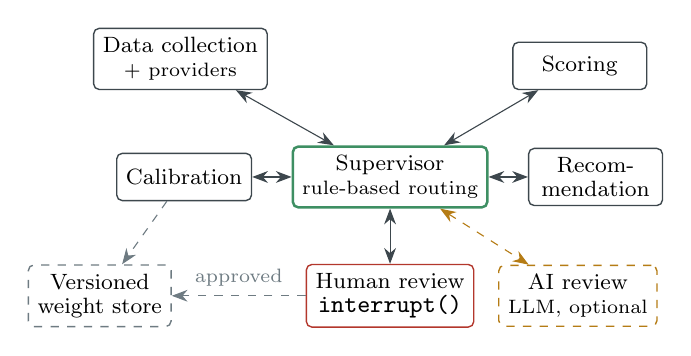
\begin{tikzpicture}[
      font=\footnotesize, >={Stealth[length=2mm]},
      node/.style={draw=ink2, rounded corners=2pt, minimum height=6mm, minimum width=17mm,
                   align=center, fill=white, line width=0.5pt},
      hub/.style={node, draw=pgreen, line width=0.9pt, minimum width=24mm},
      store/.style={node, draw=ink3, dashed}]
    \node[hub] (sup) {Supervisor\\[-1pt]{\scriptsize rule-based routing}};
    \node[node, above left=7mm and 3mm of sup] (dc) {Data collection\\[-1pt]{\scriptsize + providers}};
    \node[node, above right=7mm and 3mm of sup] (sc) {Scoring};
    \node[node, left=5mm of sup] (ca) {Calibration};
    \node[node, right=5mm of sup] (ra) {Recom-\\[-1pt]mendation};
    \node[node, below=7mm of sup, draw=pred] (hr) {Human review\\[-1pt]{\scriptsize \code{interrupt()}}};
    \node[store, left=17mm of hr] (ws) {Versioned\\[-1pt]weight store};
    \node[node, right=3mm of hr, dashed, draw=pamber, minimum width=14mm] (ar) {AI review\\[-1pt]{\scriptsize LLM, optional}};
    \foreach \n in {dc,sc,ca,ra,hr} \draw[<->, ink2] (sup) -- (\n);
    \draw[->, ink3, dashed] (ca) -- (ws);
    \draw[<->, pamber, dashed] (sup) -- (ar);
    \draw[->, ink3, dashed] (hr) -- node[above, font=\scriptsize, ink3] {approved} (ws);
  \end{tikzpicture}
  \caption{Workflow of the demonstrator. All nodes that score, calibrate, recommend and
  route are deterministic and call no language model. The dashed AI review node is entered
  only on an explicit request and interprets final results without changing them
  (Section~\ref{sec:aireview}). Every worker returns to the supervisor;
  calibration (with its re-score) and human review each run at most once per run.
  Accepted weights go to the versioned store only if auto-applied or approved.}
  \label{fig:workflow}
\end{figure}

\subsection{Scoring model}
Each factor is rated on an ordinal scale from 1 (low risk) to 5 (high risk), either by an
expert or by a rule that converts a raw indicator; an expert rating always takes
precedence, and the provenance of every rating is recorded. With effective factor weights
$\theta$ (non-negative, summing to one), dimension ratings are weighted means of their
available factors, and the overall rating $R$ is the weighted mean of the dimensions.
$R$ is mapped to a score by min-max normalisation,
\begin{equation}
  S = \frac{R-1}{4}\cdot 100 ,
\end{equation}
so that the best possible supplier scores 0, the midpoint 50 and the worst 100; a naive
$R/5$ would start at 20 and waste a fifth of the range. The mapping is affine, so rankings
are unchanged and calibration stays linear. Classes follow from thresholds on $S$ (in the
template: low $<30$, medium $<50$, high $<70$, critical from 70). Escalation rules can
raise a class but never lower it. Missing factors are excluded and the remaining weights
re-normalised; the share of weight backed by data is reported and, below a threshold,
flagged for review.

\paragraph{Sub-scores.} Dimension scores are reported alongside the overall score. Two
combine data from different origins. \textbf{Supply chain risk} combines \emph{political
stability}, from the percentile rank of the World Bank governance indicator ``Political
Stability and Absence of Violence/Terrorism'' \cite{kaufmann2011} in bands of 20 points
($\geq 80 \rightarrow 1$, \ldots, $<20 \rightarrow 5$, with a generic country risk index
as fallback), \emph{sourcing strategy} (number of qualified sources) and \emph{transport
dependency} (mode and routes). \textbf{Severity} includes \emph{change complexity}: how
long it would take to move the volume to another source, including qualification,
tooling and ramp-up. It can be derived from the \emph{time to exit} in months ($\leq 3$,
$\leq 6$, $\leq 12$, $\leq 24$, $>24$ months $\rightarrow$ 1, \ldots, 5); an expert rating still
takes precedence. Both mappings are ordinary rating sources with illustrative,
uncalibrated bands; only weights are calibrated. The default criteria, weights and
thresholds are an \textbf{illustrative template}, not a recommendation.

\subsection{Weights as objects}
The engine never reads weights from code. Each supplier receives the most specific
available weight set: calibrated weights for its material group, configured weights for
that group, calibrated global weights, or the configured defaults. Applied sets are
persisted in a versioned store and loaded at the start of the next run.

\subsection{Calibration}
For $n$ suppliers with complete ratings $\mathbf{x}_i$ and labels $y_i\in[0,100]$, the
calibrated weights solve
\begin{equation}
  \begin{gathered}
  \min_{\theta}\ \frac{1}{n}\sum_{i}\Big(\frac{s_i(\theta)-y_i}{100}\Big)^2
  + \lambda\,\lVert\theta-\theta_{\text{anchor}}\rVert^2 \\
  \text{s.t.}\quad \theta_f\geq w_{\min}\ \ \forall f, \qquad \textstyle\sum_f\theta_f=1,
  \end{gathered}
\end{equation}
with $s_i(\theta)=(\mathbf{x}_i\cdot\theta-1)/4\cdot100$ and $\theta_{\text{anchor}}$ the
configured defaults. This is a convex quadratic program, least squares with linear
constraints \cite{lawson1995}, solved by sequential least squares with an analytic
gradient. Defaults: $\lambda = 0.05\times 32/n$ (Section~\ref{sec:e2}), $w_{\min}=0.02$,
at least eight labels with complete data, and acceptance only if the cross-validated
error falls by at least 5\,\% (5 folds $\times$ 3 repeats) \emph{and} by at least two
standard errors ($z\geq2$; Section~\ref{sec:e5}). Only complete suppliers are used, since
missing-data re-weighting would make the score non-linear in $\theta$. The report also
checks for a \textbf{level offset} between labels and scores, which weights cannot
express (Section~\ref{sec:e4}); a flagged offset withholds the calibration for review.
Labels are expected as scores rather than classes, which carry less information and
would make the fit non-linear; class agreement is reported alongside the error.

\subsection{Human review}
The review step uses the graph framework's interrupt mechanism. The run is checkpointed,
and a structured request lists flagged suppliers with reasons and any proposed weights
with their metrics. The run resumes with a decision object: approved weights are stored
with the reviewer's name and the portfolio is re-scored; manual classes survive
re-scoring and are marked as overrides; recommendations are rebuilt after any change;
invalid decisions are reported and ignored.

\subsection{Two views: performance evaluation and risk management}
\label{sec:views}
Practice distinguishes two questions about the same supplier. \textbf{Performance
evaluation} looks back --- how well does the supplier deliver? --- at delivery
reliability, quality, price and responsiveness, and grades suppliers A, B or C.
\textbf{Risk management} looks forward --- how exposed are we if the supplier fails? ---
at replaceability, financial stability, supply-chain structure and compliance. The
answers can diverge: in the sample portfolio, two suppliers are critical in the risk view
and A in the performance view. The demonstrator therefore keeps both as separate
\textbf{views} on one engine; this integration is the approach's main difference from
pure risk platforms as publicly documented (Section~\ref{sec:approach}). Each criterion, with its meaning and rating source, is
defined once in a shared catalogue, and criteria such as credit risk or compliance status
serve both views. Each view has its own configuration of criteria, dimensions, weights,
classes, escalation rules and actions. Internally every view computes 0 = favourable
\ldots{} 100 = unfavourable; the performance view is only \emph{displayed} as
higher-is-better. Expert labels, weight versions, runs and reviews are kept per view, so
calibrating one view never changes the other. Everything in this section applies to each
view; the experiments in Section~\ref{sec:demo} use the risk view. In both templates
calibration is disabled by default and enabled per run; the performance view has not been
calibrated in any experiment.

\subsection{Actions, data providers and history}
\label{sec:actions}
\textbf{Action framework.} Recommendations come from three levels, all configured per
view: per class with a review cycle; per elevated dimension score; and per factor and
level with a typical owner, where the most specific level reached applies. For example,
availability of alternatives rated 4 leads to a market scan, rated 5 to qualifying an
alternative source. The actions of a portfolio form an exportable action plan; tracking
to closure is not implemented.
\textbf{Data providers.} A slim interface fills indicators missing from the supplier data
and records the origin and vintage of each value. Hand-entered values are never
overwritten, and a failing provider is reported without stopping the assessment.
Bundled are a political stability provider reading a user-downloaded table (a fictional
table, marked as such, serves the sample data), a generic provider for tabular exports
from ERP, ESG-platform or credit-agency systems, and documented placeholders for API
integrations. Providers deliver indicators only; rating stays with the rating sources, so
the method does not change when a source does.
\textbf{History.} Assessments can be recorded as timestamped snapshots per view,
explicitly or automatically after an approved review, with scores, classes, dimension
scores, weights and approver, so that suppliers and material groups can be followed over
time. Scores can be recomputed at any time; snapshots are therefore not taken on every
recalculation, which would only add noise.
\textbf{Spreadsheet surface.} A browser interface presents all of this as a sheet, with
dashboards per material group, the action plan and the history; all numbers come from the
package.

\subsection{Engineering properties}
The demonstrator ships with 159 automated tests covering scoring and weights in both
views, calibration (including recovery of known weights from noise-free labels), the
weight store and review flow, rating sources, providers, actions, reporting, history, the
interface, the consistency of the benchmark data, the reproducibility of the synthetic
datasets and the optional review agent (with mocked language-model responses only). Continuous integration runs linting and tests on two Python versions; the
checkpointer restores only allow-listed state types. The code is MIT-licensed; all data
is fictional or synthetic and labelled as such.

\subsection{Supplier Review Agent: optional, LLM-supported interpretation}
\label{sec:aireview}
One node, \code{ai\_review}, uses a language model. It is the only one, and it stands
outside the evaluation: it interprets results that the deterministic workflow has already
produced (Table~\ref{tab:aireview}).
\emph{Trigger}: only an explicit user request (a ``Generate AI Review'' button, or a
command-line option with confirmation) starts it, as a one-shot follow-up step on an
existing run; a pending human review stays pending.
\emph{Input}: one supplier's structured results from both views --- per criterion the
rating (or a gap), weight and rating basis; dimension scores, overall score and class, the
class before escalation, fired escalation rules, data completeness, missing criteria and
the rule-based actions. Supplier name, country, spend, the raw indicator record and expert
labels are not sent. The payload is shown before sending, and the node checks that it
still matches the run's results.
\emph{Output}: structured text without numeric fields --- a management summary, main
drivers (criterion and view), differences between the views, prioritised action
proposals and open questions. Scores shown with the review are copied from the
deterministic results.
\emph{Safeguards}: the whole answer is rejected if it cites a criterion not in the input,
does not compare the views, or leaves missing data without an open question; actions are
labelled as proposals for human review; each attempt is recorded in the audit trail with
a hash of the payload; failures are reported and leave the run usable.
\emph{Provider}: Anthropic's Claude, configured through environment variables; without
an API key the feature is unavailable and everything else works unchanged. The component
is experimental and unevaluated (Section~\ref{sec:limitations}).

\begin{table}[t]
  \caption{Deterministic evaluation and LLM-supported interpretation.}
  \label{tab:aireview}
  \small
  \begin{tabular}{@{}P{0.23\columnwidth}P{0.32\columnwidth}P{0.32\columnwidth}@{}}
    \toprule
     & \dimhead{Deterministic evaluation} & \dimhead{LLM-supported interpretation} \\
    \midrule
    Nodes & Data collection, scoring, calibration, recommendation, human review, supervisor & Supplier Review Agent \\
    Runs & In every run & Only on explicit request \\
    Produces & Ratings, scores, classes, weights, rule-based actions & Summary, drivers, view differences, action proposals, open questions \\
    Changes numbers & Yes, recomputably & No; numbers are copied \\
    Reproducible & Same input, same output & No; output can vary \\
    Tested & Unit and flow tests & Mocked responses on synthetic suppliers; quality not evaluated \\
    \bottomrule
  \end{tabular}
\end{table}

% ═══════════════════════════════════════════════════════════════════════
\section{Demonstration on synthetic data}
\label{sec:demo}

All numbers in this section are produced by deterministic scripts in the repository,
run on commit \code{6bb05b9} and re-checked on \code{c9a500f}; the tables behind every
figure are in \code{docs/paper/results/}. \textbf{Scope of the evidence:} the data is
synthetic throughout. Every ``expert label'' in E1--E5 is generated by a constructed expert
policy; no real category manager provided labels, and no result has been validated in the
field. The experiments show how the procedure behaves under known conditions, not how well
it works in practice.

\subsection{Design}
\textbf{Generator.} Synthetic suppliers are drawn with random ratings and indicators.
Each receives an ``expert label'': its score under a \textbf{hidden weighting}, plus
Gaussian noise ($\sigma=4$), rounded to steps of five as category managers tend to state
judgements, and clipped to $[0,100]$. The hidden weighting differs from the template:
the simulated experts care more about business impact (22\,\% instead of 14\,\%) and
single sourcing (16\,\% instead of 8.75\,\%) and less about the ESG rating (3\,\% instead
of 12\,\%). Noise and rounding imply an \textbf{irreducible error of 18.1~\ptsq} (noise
floor) that no model can beat out of sample. Because the generating weights are known,
calibration can be judged on whether it reduces error out of sample, whether it moves the
weights towards the truth, and how both depend on $\lambda$ and $n$.
\textbf{Data.} A reference portfolio of 36 suppliers (32 labelled), shipped with the
repository; training draws of 8--192 labels (30 seeds per size, plus 100 seeds at
$n=32$); and an independent test set of 2{,}000 suppliers, scored also against
noise-free true scores to isolate estimation error.
\textbf{Experiments.} E1: repeated 5-fold cross-validation \cite{stone1974,kohavi1995} on
the reference portfolio over $\lambda$; E2: sample size $\times\,\lambda$ on the test set; E3: weight stability
over 100 seeds; E4: misspecified expert policies; E5: the acceptance threshold.

\subsection{Reference run}
On the reference portfolio with $\lambda=0.05$, the error between score and label falls
from 37.8 to 13.3~\ptsq, class agreement rises from 84\,\% to 88\,\%, the L1 distance to the
hidden weighting falls from 0.345 to 0.138, and re-scoring with the calibrated weights (applied only
after approval under the current risk template) changes the class of 2 of 36 suppliers. The
acceptance rule accepts the calibration on an out-of-fold error of 37.8~$\rightarrow$~22.8
($z=2.4$). The in-sample 13.3 lies \emph{below} the noise floor: ten weights fitted to 32
noisy labels partly fit the noise. E1 quantifies by how much.

\subsection{Out-of-sample error and the choice of \texorpdfstring{$\lambda$}{lambda} (E1)}

\begin{table}[t]
  \caption{E1: repeated 5-fold cross-validation on the reference portfolio (32 labels, 20
  repeats). MSE in \ptsq; noise floor 18.1; default weights: 37.8 out of fold and 84\,\%
  out-of-fold class agreement. $\pm$: standard deviation across repeats. \synth}
  \label{tab:e1}
  \small
  \setlength{\tabcolsep}{4.5pt}
  \begin{tabular}{@{}rrrrr@{}}
    \toprule
    $\lambda$ & CV MSE & in-sample & class agr. & L1 to hidden \\
    \midrule
    0 & $22.9\pm4.2$ & 10.0 & 81\,\% & 0.155 \\
    0.02 & $20.8\pm2.7$ & 10.7 & 83\,\% & 0.142 \\
    \textbf{0.05} & $\mathbf{20.6\pm2.0}$ & 12.4 & 86\,\% & 0.163 \\
    0.2 & $24.4\pm1.2$ & 18.9 & 84\,\% & 0.241 \\
    1 & $32.3\pm0.5$ & 29.9 & 84\,\% & 0.309 \\
    5 & $36.4\pm0.1$ & 35.8 & 84\,\% & 0.337 \\
    \bottomrule
  \end{tabular}
\end{table}

\begin{figure}[t]
  \centering
  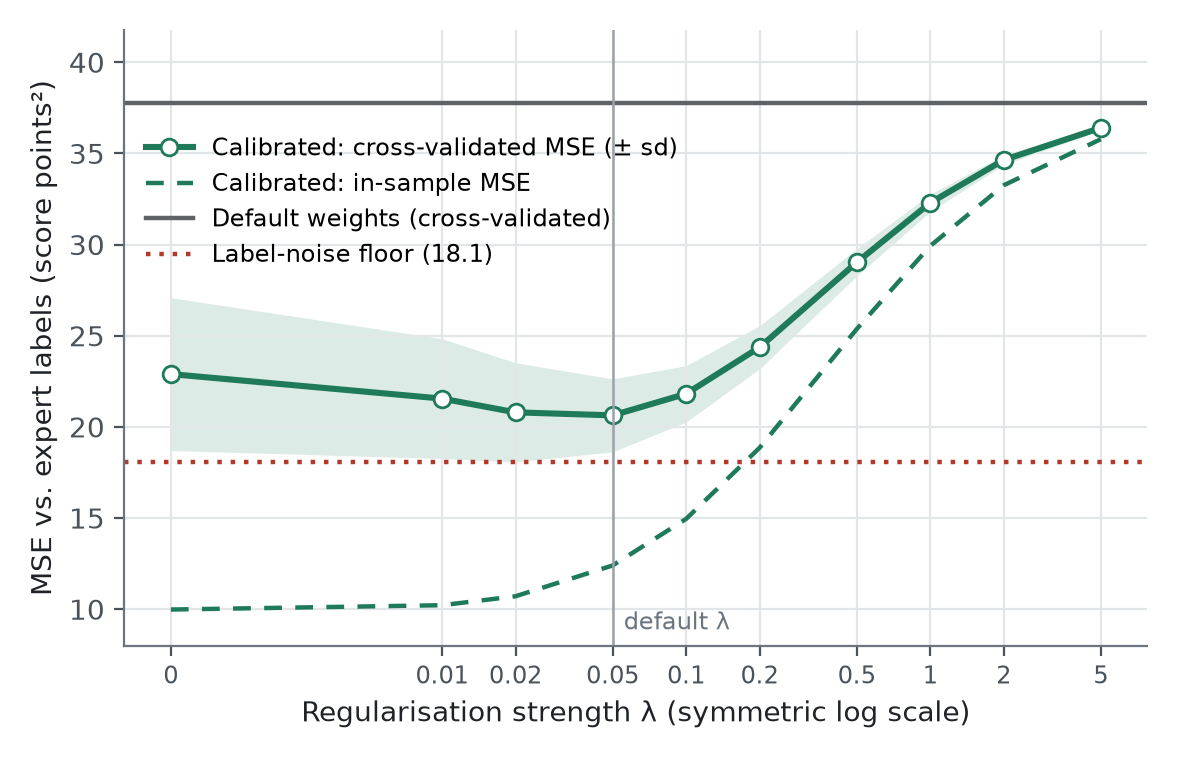
\includegraphics[width=\columnwidth]{figures/fig04_lambda_curve.png}
  \caption{Cross-validated and in-sample MSE of calibrated weights versus $\lambda$ on the
  reference portfolio. Horizontal lines: cross-validated error of the default weights and
  the irreducible label noise. The gap between the solid and dashed lines is the
  in-sample optimism. \synth}
  \label{fig:lambda}
\end{figure}

Calibration generalises (Table~\ref{tab:e1}, Figure~\ref{fig:lambda}): at $\lambda=0.05$
the cross-validated error falls from 37.8 to 20.6, a 45\,\% reduction within 2.5~\ptsq{}
of the noise floor, while the in-sample error overstates the gain by about 8~\ptsq. The
default lies at the bottom of the curve, but it was set before this experiment on data
from the same generator, so this is consistency, not proof. Regularisation buys stability
more than accuracy: from $\lambda=0$ to $0.05$ the mean improves modestly and its spread
halves; strong regularisation gives up most of the gain. Error and class agreement can
diverge: without regularisation, out-of-fold class agreement \emph{falls} below the
default (81\,\% vs.\ 84\,\%) although the error improves --- which is why both are
reported.

\subsection{How many labels, and how strongly to regularise (E2)}
\label{sec:e2}
Against the noise-free true scores, the default weights have a structural error of
29.7~\ptsq{} (Table~\ref{tab:e2}, Figure~\ref{fig:learning}).

\begin{table}[t]
  \caption{E2: test error against true scores (mean over 30 seeds; default weights 29.7)
  and, in brackets, the share of seeds in which calibration beats the defaults. Fixed
  $\lambda$, the scaled default $0.05\times32/n$, and $\lambda$ chosen by cross-validation
  with the minimum-error rule. \synth}
  \label{tab:e2}
  \small
  \setlength{\tabcolsep}{2.4pt}
  \begin{tabular}{@{}rllll@{}}
    \toprule
    $n$ & $\lambda=0$ & $\lambda=0.05$ & \textbf{scaled} & CV min \\
    \midrule
    8 & 37.7 (50\,\%) & 16.7 (90\,\%) & \textbf{18.4 (100\,\%)} & 24.5 (90\,\%) \\
    16 & 16.2 (90\,\%) & 9.9 (100\,\%) & \textbf{11.5 (100\,\%)} & 12.8 (100\,\%) \\
    32 & 6.1 (100\,\%) & 5.9 (100\,\%) & \textbf{5.9 (100\,\%)} & 5.6 (100\,\%) \\
    64 & 2.8 (100\,\%) & 4.2 (100\,\%) & \textbf{3.0 (100\,\%)} & 3.0 (100\,\%) \\
    192 & 0.8 (100\,\%) & 2.5 (100\,\%) & \textbf{0.8 (100\,\%)} & 0.8 (100\,\%) \\
    \bottomrule
  \end{tabular}
\end{table}

\textbf{Small samples need regularisation.} With eight labels and no regularisation,
calibration is \emph{worse} than the defaults on average (37.7 vs.\ 29.7) and wins in only
half of the seeds; with $\lambda=0.05$ the same labels nearly halve the error and win in
90\,\%. At 32 labels the default removes about 80\,\% of the structural error
(29.7~$\rightarrow$~5.9). \textbf{A fixed $\lambda$ becomes a bias at large $n$}: beyond
about 48 labels the unregularised fit is better (0.8 vs.\ 2.5 at $n=192$), because the
error term is a mean over suppliers while the penalty is not scaled. \textbf{Scaling
$\lambda$ with $1/n$} --- a prior of constant strength, anchored at $\lambda=0.05$ for 32
labels --- removes this bias (0.76 vs.\ 0.78 at $n=192$), beats the defaults in every
seed from eight labels upwards, and under the default acceptance rule caused no harmful
acceptance at any size. Choosing $\lambda$ by cross-validation was tested and not
adopted: the one-standard-error rule \cite{hastie2009} over-regularises in the middle
range (10.6 vs.\ 5.9 at 32 labels), the minimum-error rule is too noisy with few labels
(24.5 vs.\ 18.4 at eight), and both cost an order of magnitude more computation. The
scaling constant was itself set on the same synthetic data; it is a reasoned default.

\begin{figure*}[t]
  \centering
  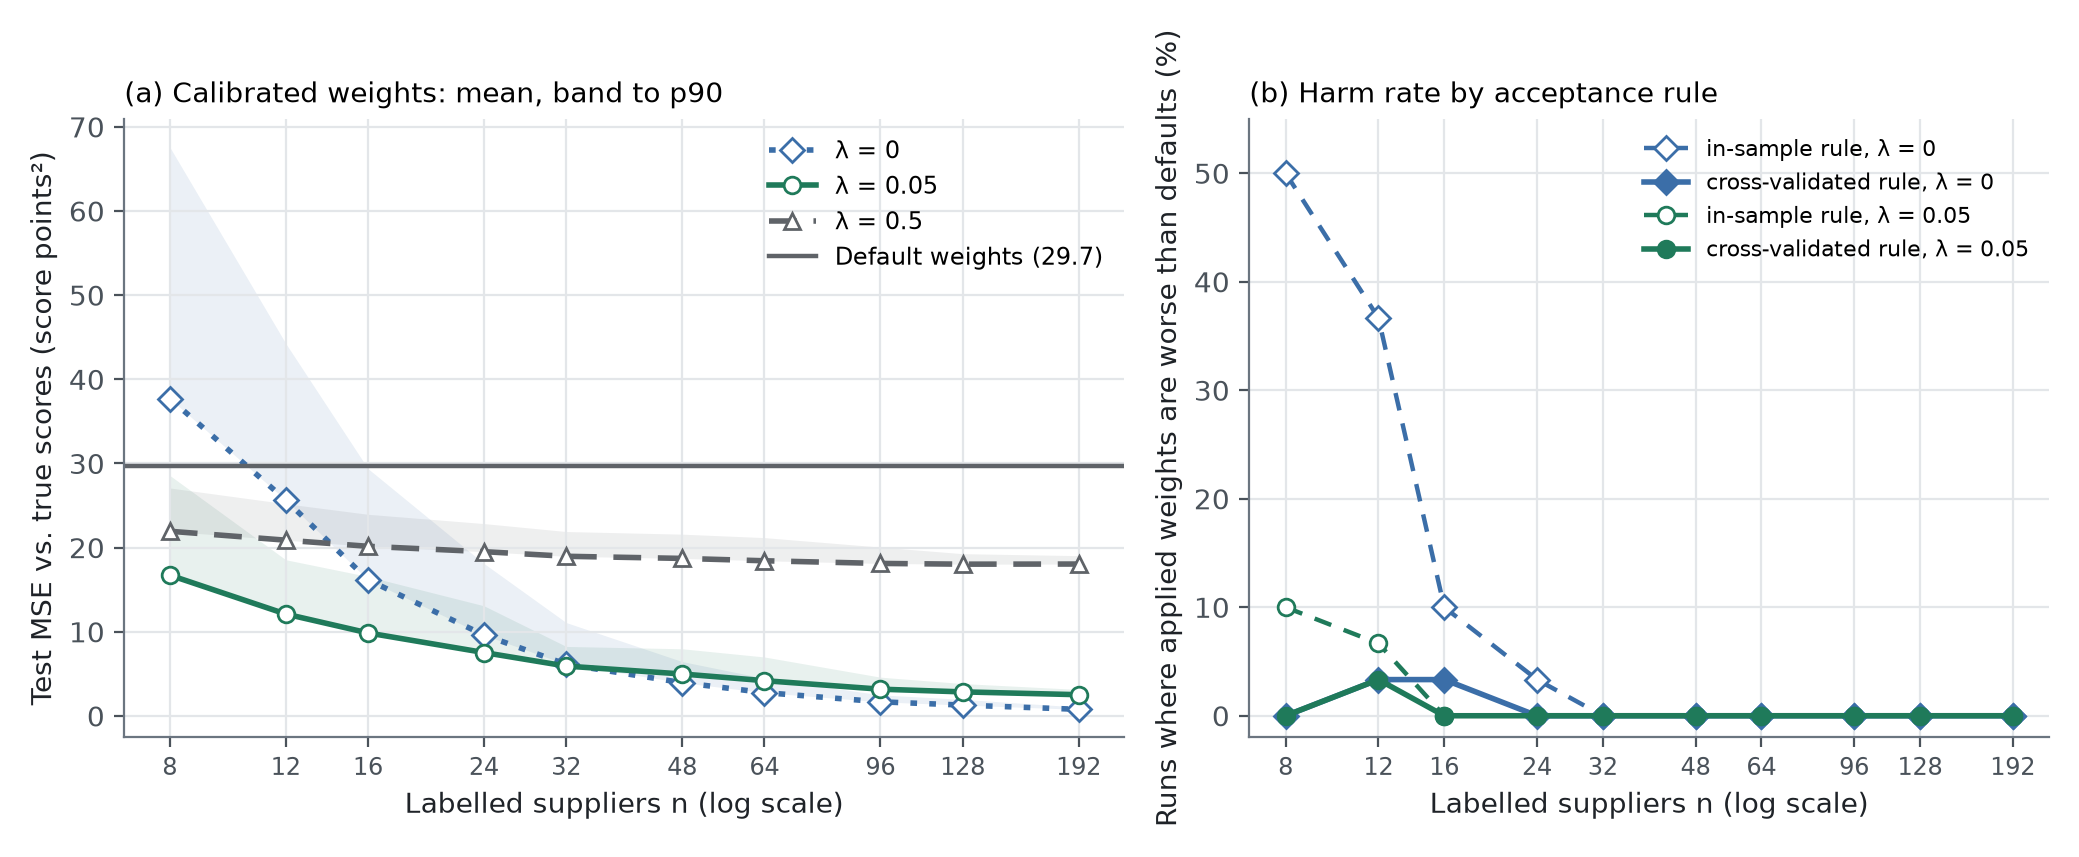
\includegraphics[width=0.92\textwidth]{figures/fig05_learning_curve.png}
  \caption{(a) Test error of calibrated weights against noise-free true scores, by number
  of labels, for fixed $\lambda$, the scaled default and $\lambda$ chosen by
  cross-validation (mean over 30 seeds; band to the 90th percentile). (b) Share of runs in
  which the weights actually applied are worse than the defaults, under the in-sample rule
  and the default cross-validated rule (5\,\% and $z\geq2$). \synth}
  \label{fig:learning}
\end{figure*}

\subsection{Stability of the recovered weights (E3)}
Across 100 portfolios of 32 labels ($\lambda=0.05$), the mean L1 distance to the hidden
weighting is 0.170, against 0.345 for the defaults (Figure~\ref{fig:stability}). Large
deviations are recovered reliably: business impact (14\,\%~$\rightarrow$~22\,\%,
calibrated mean 19.5\,\%), sourcing strategy (8.75\,\%~$\rightarrow$~16\,\%, 14.1\,\%) and
ESG rating (12\,\%~$\rightarrow$~3\,\%, 6.3\,\%) move in the right direction in all 100
seeds. Small deviations are not: for two factors whose default and hidden weights differ
by half a percentage point, the direction is right in only 67 and 54 seeds, close to
chance. Estimates are shrunk towards the default as intended; large shifts are recovered
at roughly two-thirds of their size.

\begin{figure}[t]
  \centering
  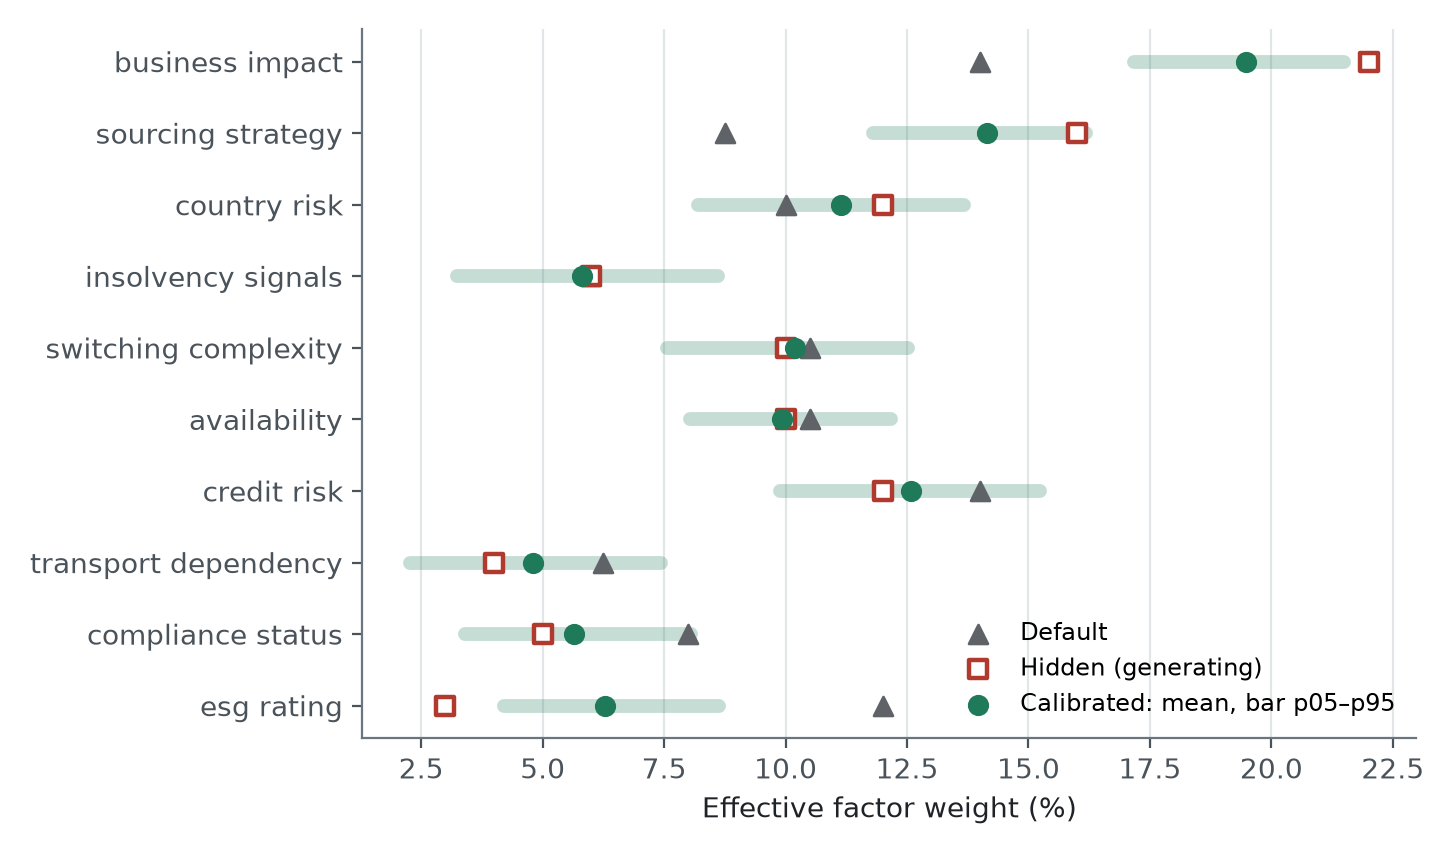
\includegraphics[width=\columnwidth]{figures/fig06_weight_stability.png}
  \caption{Effective factor weights: configured default, hidden weighting, and calibrated
  weights (mean and 5th--95th percentile over 100 portfolios of 32 labels,
  $\lambda=0.05$). \synth}
  \label{fig:stability}
\end{figure}

\subsection{Acceptance rules: in-sample versus cross-validated}
\label{sec:acceptance}
The demonstrator originally accepted calibrated weights if they reduced the
\emph{in-sample} error by at least 5\,\%. In E1--E3 this rule accepted practically every
calibration, including the eight-label, unregularised runs in which the weights were worse
than the defaults in half of the seeds. \textbf{An in-sample rule is not a safeguard
against overfitting}; it only protects against calibrations that change nothing. It was
replaced by an out-of-sample test: refit on $k-1$ folds, evaluate on the held-out fold,
repeat with reshuffled folds (5 $\times$ 3, deterministic), and require the pooled
out-of-fold error to improve by at least 5\,\%. Table~\ref{tab:acceptance} reports this
5\,\% rule (commit \code{ddcb977}); Section~\ref{sec:e5} adds the second condition that
is now the default.

\begin{table}[t]
  \caption{In-sample versus 5\,\% cross-validated acceptance on the E2 runs (30 seeds;
  error against true scores; defaults 29.7). Harm: share of runs in which the weights in
  use are worse than the defaults. \synth}
  \label{tab:acceptance}
  \small
  \setlength{\tabcolsep}{4pt}
  \begin{tabular}{@{}rrccc@{}}
    \toprule
    $n$ & $\lambda$ & accepted & error in use & harm \\
     & & in-s.\ / CV & in-s.\ / CV & in-s.\ / CV \\
    \midrule
    8 & 0 & 100 / 23\,\% & 37.7 / 30.8 & 50 / 7\,\% \\
    8 & 0.05 & 100 / 57\,\% & 16.7 / 20.8 & 10 / 3\,\% \\
    12 & 0 & 100 / 47\,\% & 25.7 / 27.7 & 37 / 20\,\% \\
    12 & 0.05 & 100 / 70\,\% & 12.1 / 16.3 & 7 / 3\,\% \\
    16 & 0.05 & 100 / 87\,\% & 9.9 / 11.8 & 0 / 0\,\% \\
    $\geq24$ & 0.05 & 100 / 100\,\% & identical & 0 / 0\,\% \\
    \bottomrule
  \end{tabular}
\end{table}

The cross-validated rule sharply reduces harm where harm occurs (50\,\% to 7\,\% at eight
unregularised labels). It is conservative: with few labels it also rejects helpful
calibrations, so the error of the weights in use is higher than under the in-sample rule
(20.8 vs.\ 16.7 at $n=8$), though still well below the defaults. It trades expected gain
for a lower risk of making things worse --- the appropriate trade-off for weights that
drive supplier decisions. From about 24 labels both rules agree. On the shipped data,
the rule changes one visible outcome: a calibration restricted to the ten labelled
``plastics'' suppliers looked excellent in-sample (36.8~$\rightarrow$~10.4) but was worse
out of sample (36.8~$\rightarrow$~41.7) and is now rejected. Group-specific calibration
needs enough labels per group.

\subsection{When experts do not judge like the model (E4)}
\label{sec:e4}
E1--E3 generate labels from the linear model family that calibration fits: the best case.
E4 replaces that policy with alternatives a real panel might follow: more or less noise,
coarser rounding, a uniform level shift (10 points stricter), an interaction between
business impact and single sourcing, a knock-out floor (a severe compliance or insolvency
rating lifts the judgement to at least 70), a non-compensatory ``worst factor dominates''
policy, and two experts with different weightings. For each policy, an
\textbf{approximation floor} --- the error of the best constrained linear weighting on
2{,}000 noise-free judgements --- measures how far it lies outside what weights can
express. Calibration then runs with production settings on 16, 32 and 64 labels, 30 seeds
each (Table~\ref{tab:e4}, Figure~\ref{fig:robustness}).

\begin{table*}[t]
  \caption{E4: calibration under misspecified expert policies. Errors in \ptsq{} against
  the policy's noise-free judgement, ``calibrated'' at $n=32$. Excess removed: share of
  the default weights' error above the linear floor that calibration removes, at
  $n=16/32/64$. Harm: share of runs with weights in use worse than the defaults, at
  $n=16/32$. Original: fixed $\lambda=0.05$ and the 5\,\% rule; current: scaled
  $\lambda$ and the rule with $z\geq2$. \synth}
  \label{tab:e4}
  \footnotesize
  \setlength{\tabcolsep}{4.5pt}
  \begin{tabular}{@{}lrrrllllc@{}}
    \toprule
    Policy & floor & default & calibrated & \multicolumn{2}{c}{excess removed} & \multicolumn{2}{c}{harm} & class agreement \\
    \cmidrule(lr){5-6}\cmidrule(lr){7-8}
     & & & & original & current & original & current & default\,$\rightarrow$\,cal. \\
    \midrule
    linear (reference) & 0 & 29.7 & 5.7 & 69 / 81 / 87\,\% & 62 / 81 / 91\,\% & 0 / 0\,\% & 0 / 0\,\% & 79\,$\rightarrow$\,91\,\% \\
    linear, $\sigma=8$ & 0 & 29.7 & 11.7 & 30 / 61 / 75\,\% & 39 / 61 / 76\,\% & 7 / 0\,\% & 0 / 0\,\% & 79\,$\rightarrow$\,87\,\% \\
    linear, steps of 10 & 0 & 29.7 & 7.0 & 63 / 76 / 84\,\% & 58 / 76 / 88\,\% & 0 / 0\,\% & 0 / 0\,\% & 79\,$\rightarrow$\,90\,\% \\
    level shift $+10$ & 62.3 & 157.4 & 77.6 & 74 / 84 / 90\,\% & 77 / 84 / 91\,\% & 0 / 0\,\% & 0 / 0\,\% & 44\,$\rightarrow$\,60\,\% \\
    interaction & 71.9 & 103.1 & 88.0 & 9 / 48 / 68\,\% & 24 / 48 / 66\,\% & 10 / 0\,\% & 0 / 0\,\% & 63\,$\rightarrow$\,65\,\% \\
    knock-out floor & 98.3 & 127.0 & 118.8 & $-24$ / 28 / 62\,\% & 8 / 28 / 58\,\% & 10 / 13\,\% & 0 / 3\,\% & 66\,$\rightarrow$\,69\,\% \\
    worst factor dominates & 284.3 & 418.0 & 328.1 & 57 / 67 / 82\,\% & 69 / 67 / 78\,\% & 0 / 0\,\% & 0 / 0\,\% & 12\,$\rightarrow$\,27\,\% \\
    two experts disagree & 0 & 5.3 & 5.3 & $-84$ / 1 / 42\,\% & $-22$ / 1 / 29\,\% & 43 / 23\,\% & 0 / 0\,\% & 90\,$\rightarrow$\,91\,\% \\
    \bottomrule
  \end{tabular}
\end{table*}

\begin{figure*}[t]
  \centering
  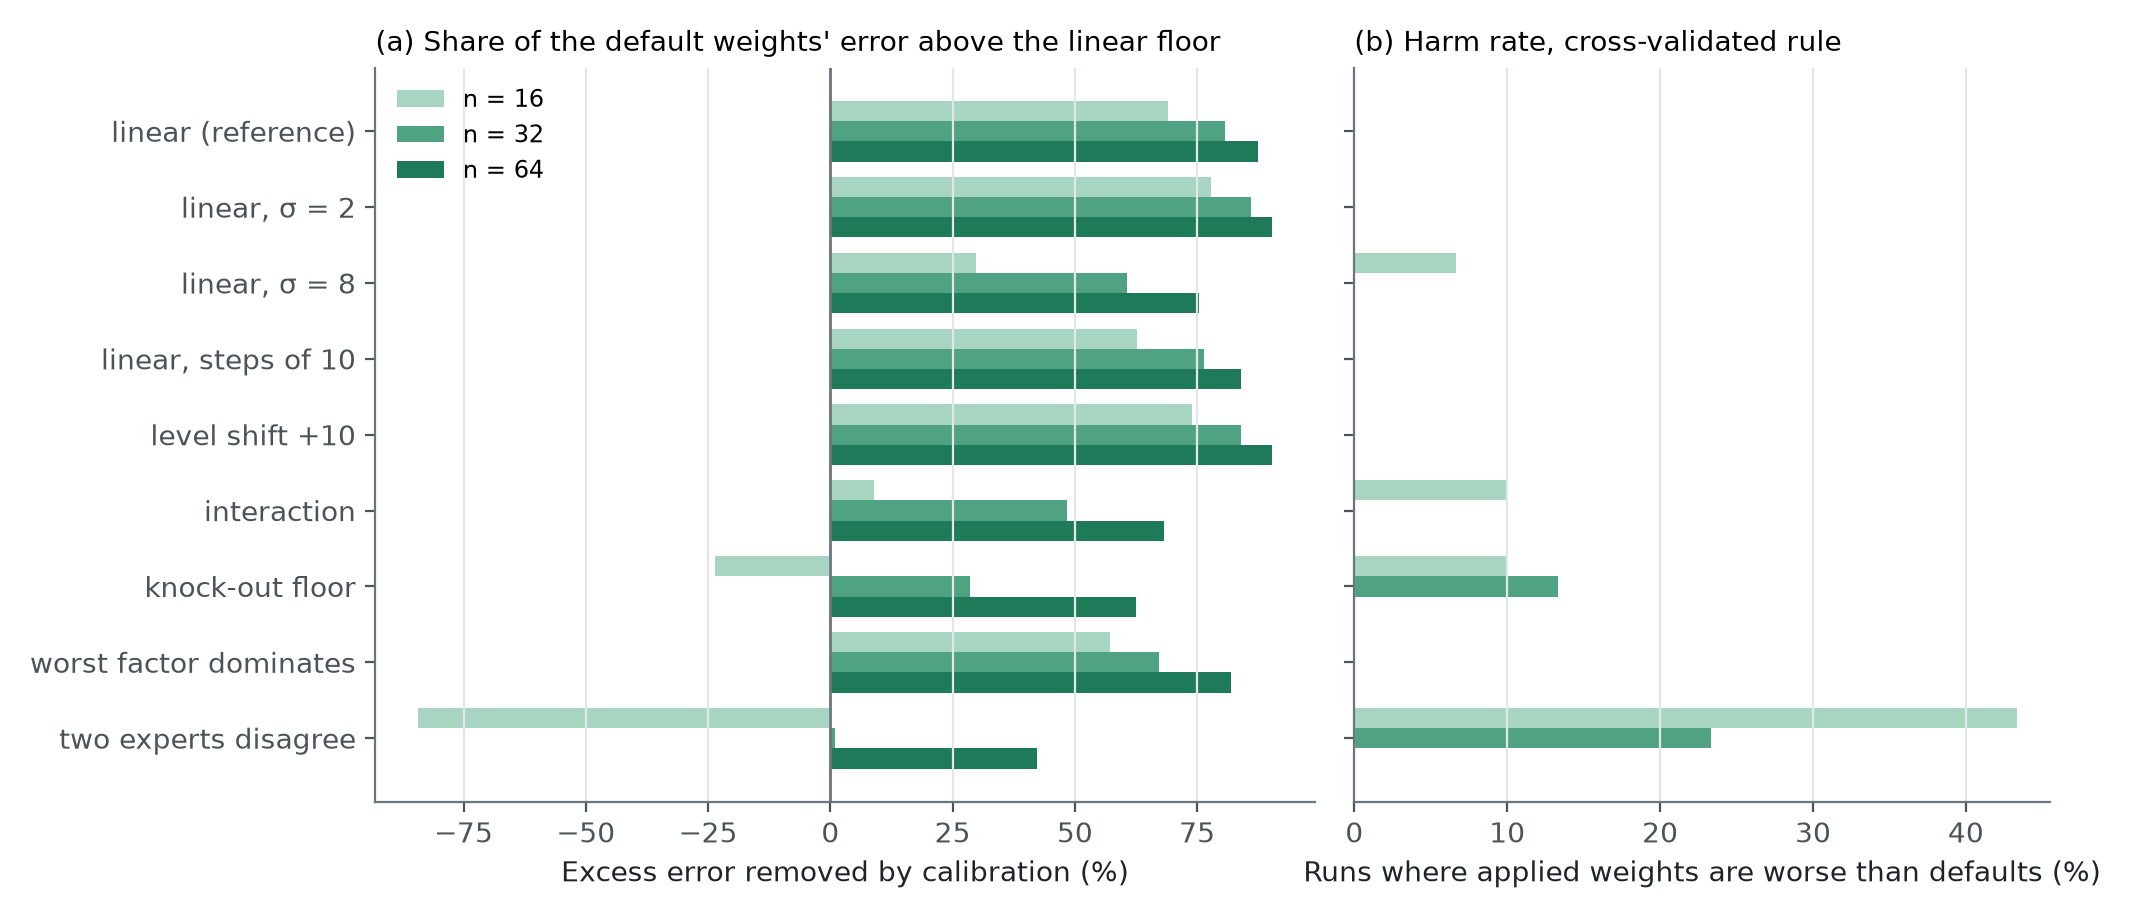
\includegraphics[width=0.92\textwidth]{figures/fig07_robustness.png}
  \caption{(a) Share of the default weights' excess error above the linear floor that
  calibration removes, by expert policy and number of labels. (b) Share of runs in which
  the weights in use are worse than the defaults under the default rule (5\,\% and
  $z\geq2$); almost all bars are zero. \synth}
  \label{fig:robustness}
\end{figure*}

\textbf{Noise and rounding cost labels, not validity}: with linear experts, calibration
stays effective under coarse rounding and doubled noise, but needs more labels.
\textbf{Non-linear policies leave a floor no weighting removes}: for the interaction,
knock-out and worst-factor policies, calibration closes much of the gap above the floor
with 32--64 labels, but class agreement barely improves. Weights cannot learn a policy
that is not additive, and a large remaining error should be reported as exactly that
signal. \textbf{Knock-outs belong in escalation rules, not in weights}: with sixteen
labels and a fixed $\lambda$, calibration is worse than the defaults on average, and even
the 5\,\% rule lets 10--13\,\% of runs end with harmful weights (0--3\,\% under the current
default, mostly because such calibrations are no longer accepted). The demonstrator's
escalation rules are the right mechanism; knock-outs should be \emph{elicited} from
category managers and encoded as rules. \textbf{A level offset cannot be expressed by
weights}, which sum to one. Calibration then distorts the weights to imitate the offset:
weight moves towards factors that are usually rated high (the shift correlates at 0.89
with the factor's mean rating), and insolvency signals and compliance status --- the rare,
severe drivers a risk model should protect most --- are pushed to the minimum. The
demonstrator now diagnoses this: it flags a mean difference of at least 5 points that is
also two standard errors from zero and withholds such calibrations for review. The flag
caught every level-shift and worst-factor run, 30--37\,\% of knock-out runs, at most
7\,\% of purely linear runs at sixteen labels and none from 32. \textbf{Disagreeing
experts are the hardest case}: their disagreement acts as structured label noise, and the
5\,\% rule accepted harmful weights in 43\,\% of runs at sixteen labels --- the
motivation for E5.

\textbf{Fit diagnostics.} Since knock-outs and non-additive judgement cannot be fixed by
weights, the report says when they are likely, without blocking approval. A \emph{high
residual} (cross-validated error at least 40\,\% of the label variance) detects 63--100\,\%
of non-linear runs and 0--7\,\% of linear ones. A \emph{knock-out candidate} (at least
three suppliers with a severe rating judged at least 5 points and two standard errors
riskier than the model predicts, after removing the offset) found the knock-out policy in
13/53/97\,\% of runs at $n=16/32/64$, always on the right factor family, with at most
3\,\% false hints from linear experts (7\,\% with very noisy labels). A factor \emph{pushed to the minimum weight} is
reported only as ``check this factor'': it is unspecific. None of the hints detects
expert disagreement reliably. E4 thus maps where calibration works (noisy but broadly
additive judgement), where it is partial (non-additive policies) and where it fails
(knock-outs, level offsets, disagreement) --- but it cannot say which policy real category
managers follow.

\subsection{Requiring a clear improvement (E5)}
\label{sec:e5}
A fixed 5\,\% threshold cannot tell a real improvement from a lucky one when the
estimate itself is noisy. The acceptance rule therefore has a second condition.
Cross-validation yields an out-of-fold error for every labelled supplier under the active
weights and under refitted weights; from the per-supplier differences the rule computes the
mean improvement and its standard error, whose ratio $z$ must reach a threshold. This
standard error is optimistic, because out-of-fold errors are not independent
\cite{nadeau2003,bengio2004}; $z$ is a screening statistic, not a test with a nominal
error rate, and the threshold was chosen \textbf{empirically}. E5 covers 20 scenarios
(five expert policies $\times$ 8/16/32/64 labels), seven thresholds and 100 seeds each,
with the scaled $\lambda$ (Table~\ref{tab:e5}).

\begin{table}[t]
  \caption{E5: effect of the uncertainty threshold, averaged over 20 scenarios (100 seeds
  each). Missed gain: error of the weights in use minus the better of default and
  calibrated weights, as a share of the default error. Rel.\ error: error of the weights in
  use divided by the default error. \synth}
  \label{tab:e5}
  \small
  \setlength{\tabcolsep}{2.8pt}
  \begin{tabular}{@{}lcrrr@{}}
    \toprule
    $z\geq$ & harm & accepted & missed & rel.\ \\
     & mean / worst & & gain & error \\
    \midrule
    0 (5\,\%) & 7.4 / 30\,\% & 61\,\% & 10.1\,\% & 0.78 \\
    1 & 4.2 / 17\,\% & 46\,\% & 12.4\,\% & 0.80 \\
    1.5 & 2.2 / 8\,\% & 34\,\% & 15.2\,\% & 0.83 \\
    \textbf{2 (default)} & \textbf{1.1 / 4\,\%} & 24\,\% & 18.7\,\% & 0.87 \\
    2.5 & 0.4 / 3\,\% & 15\,\% & 22.2\,\% & 0.90 \\
    3 & 0.1 / 1\,\% & 10\,\% & 25.1\,\% & 0.93 \\
    \bottomrule
  \end{tabular}
\end{table}

The selection criterion was the \emph{smallest threshold for which no scenario exceeds
5\,\% harmful acceptances}: $z\geq2$. Against the 5\,\% rule alone, it gives up about nine
percentage points of the default error in expected improvement (0.78~$\rightarrow$~0.87)
for a worst-case harm rate that falls from 30\,\% to 4\,\%. Re-run with the new default,
harm falls to zero for disagreeing experts (from 43/23\,\% at 16/32 labels), to 0/3\,\% for
knock-outs, and to 0\,\% at every size in E2 with the scaled $\lambda$; the reference
portfolio is still accepted ($z=2.4$). \textbf{Calibration now has to be earned}: with
linear experts, 17\,\% of calibrations are applied at 8 labels, 50\,\% at 16 and 87\,\% at
32; with disagreeing experts, none at 16 or 32. When it withholds a calibration, the rule
keeps the defaults and states why. For practice this means roughly \textbf{30 or more
consistent labels per calibration scope}, and measuring expert agreement before calibrating
a scope with several labelling experts. A rule that sometimes forgoes an improvement is
the right failure mode for weights that drive supplier decisions; a rule that sometimes
makes them worse is not. The threshold was selected and evaluated on the same synthetic
scenarios and should be treated as a reasoned default.

\subsection{What the demonstration shows, and what it does not}
Under controlled conditions, the procedure generalises close to the noise floor,
recovers the direction and roughly the size of substantial weight differences, needs
regularisation when labels are few, and shows the user in-sample figures that are
optimistic by a quantifiable margin. It does not show how real expert judgement behaves:
E1--E3 use best-case labels, and E4 cannot say which policy describes real category
managers or whether it changes over time. Policy-capturing research suggests that linear
models often describe holistic judgements well \cite{karelaia2008}; whether this holds for
supplier-risk judgements is an empirical question. The demonstration also says nothing
about \textbf{predictive validity}.

% ═══════════════════════════════════════════════════════════════════════
\section{Comparison and discussion}
\label{sec:discussion}

\subsection{What the benchmark and the demonstrator show together}
The benchmark locates a gap rather than a winner. Spreadsheets keep the method in the
procurement team's hands but cannot hold it to account; platforms bring data, scale and
operational maturity but keep the method partly or largely outside the customer's view;
open-source agent projects offer architecture, with little emphasis on a scoring method.
In the author's qualitative assessment, no approach is strong both on \emph{data coverage}
and on \emph{ownership of the method}, and none of the established ones documents
publicly an evaluation of risk and performance on one basis. The demonstrator shows that
the method layer can be built lean and can carry both views: deterministic and tested,
orchestrated by deterministic, specialised agents over a shared state (no language
model in scoring, calibration, recommendations or routing), governed by a real pause and
versioned approvals, able to learn under a cross-validated acceptance test, with risk
management, performance evaluation and an action framework from one catalogue --- in a
small, MIT-licensed code base. What
neither part shows is that real category managers judge in a way a linear model can
capture, that calibrated scores predict disruptions, or that the approach scales
operationally to an enterprise portfolio.

\subsection{The hybrid reading: signals from outside, method in-house}
\label{sec:hybrid}
The most useful reading of Figure~\ref{fig:profile} is not ``which approach is best''
but ``which layer each approach should provide'' (Table~\ref{tab:layers}). In this
reading the demonstrator does not compete with a platform; it \emph{consumes} one. The
integration points exist: rating sources turn any indicator, including a platform score,
an alert count or a country index, into a 1--5 rating; a pluggable data source delivers
indicators; and data providers fill missing indicators with recorded origin --- the
political stability provider is a small instance of a signal layer built on open data.
Three consequences follow. \emph{Platform scores become inputs, not verdicts}: procurement
decides, and calibrates, how much they count per material group, and the class remains
recomputable. \emph{Double counting must be managed}: a platform score that already
contains country risk overlaps with a separate country factor; either one is dropped or
calibration is left to down-weight it, which works only with enough labels.
\emph{Licence terms matter}: whether platform scores may be stored, versioned and
recomputed in-house depends on the contract, which this paper did not examine.

\begin{table}[t]
  \caption{A layered reading of supplier risk evaluation.}
  \label{tab:layers}
  \small
  \begin{tabular}{@{}P{0.14\columnwidth}P{0.36\columnwidth}P{0.37\columnwidth}@{}}
    \toprule
    \dimhead{Layer} & \dimhead{Question} & \dimhead{Strong here / suggested provider} \\
    \midrule
    Signal & What is happening to this supplier, its country, its tier-N network, now? & Platforms (signals, coverage); subscription or open data (governance indicators, sanction lists, insolvency registers) \\
    Method & How do signals and internal knowledge become a class, with which weights, and why? & Lean Agentic (transparency, calibration, group weights); in-house, owned by procurement \\
    Decision & What do we do about it, and who decides? & Shared; category managers and a named decision owner, see Section~\ref{sec:governance} \\
    \bottomrule
  \end{tabular}
\end{table}

\subsection{When which approach fits}
Because the profiles are not ranked, the choice depends on the situation. A
\emph{spreadsheet with discipline} --- written definitions, versioned weights, a fixed
review date --- is adequate for a small portfolio with stable risk drivers and no
documentation duty. A \emph{commercial platform} is hard to replace where tier-N exposure,
real-time monitoring or regulatory evidence dominate; building that coverage in-house is
neither lean nor realistic. A \emph{Lean Agentic method layer} fits organisations that
have outgrown the spreadsheet, want to own and justify their method, need material-group
weighting and want their category managers' judgement to shape the model --- also
alongside a platform. For a mid-sized procurement organisation, the most likely
configuration is the combination.

\subsection{The cost of being lean}
``Lean'' and ``open source'' do not mean free. Cost shifts from licences to ownership
(someone maintains configuration, code and data connections), skills (a configuration file
to change the method, Python to extend the system) and responsibility (no vendor, no
service levels, no security hardening; operational maturity is rated 2). The approach is
lean in what it \emph{builds}, not necessarily in what it \emph{requires} to run.

\subsection{What the ``agentic'' part contributes}
Scoring, calibration, recommendations and routing use no language model at all; the one
language-model component, the optional review agent, interprets results after the fact
(Section~\ref{sec:aireview}). For the current
scope, the agent architecture is not strictly necessary; the same logic could run as a
pipeline. It pays off as the system grows: the supervisor routes bounded loops explicitly,
foreseeable additions (an external-signal agent, a document-extraction agent, an
explanation agent) become new nodes rather than rewrites --- the review agent is a first,
experimental instance of the last, added as one node without changing the others --- and checkpointing provides the
pause-and-resume that human review needs. The value of ``agentic'' here is
\textbf{orchestration and extensibility, not autonomy}: authority over scores and
decisions stays with code that can be recomputed and with people who can be named.

% ═══════════════════════════════════════════════════════════════════════
\section{Governance and decision ownership}
\label{sec:governance}

A risk score does not decide anything; it informs a decision made by someone accountable
for it. Table~\ref{tab:ownership} proposes how roles could be assigned; the demonstrator
does not enforce them.

\begin{table*}[t]
  \caption{Proposed ownership of the elements of the method.}
  \label{tab:ownership}
  \small
  \begin{tabular}{@{}P{0.245\textwidth}P{0.20\textwidth}P{0.19\textwidth}P{0.27\textwidth}@{}}
    \toprule
    \dimhead{Element} & \dimhead{Owner (proposed)} & \dimhead{Changed how} & \dimhead{Recorded where} \\
    \midrule
    Criteria, scales, default weights, thresholds, escalation rules & Method owner (e.g.\ procurement excellence) & Reviewed configuration change, new model version & Version control; model version on every result \\
    Expert ratings per supplier & Category manager & During the supplier review & Supplier record; rating provenance per factor \\
    Holistic labels for calibration & Category managers, blind to the model score & Periodic labelling round & Supplier record \\
    Calibrated weights & Approver distinct from the label providers & Approval at the review pause & Versioned weight store with approver, metrics, timestamp \\
    Manual class overrides & Decision owner for the supplier & Review decision with mandatory comment & Assessment; audit trail \\
    Indicators from external sources & Data owner per source & Data refresh & Provider and data vintage per indicator; source data not versioned \\
    \bottomrule
  \end{tabular}
\end{table*}

Two principles follow. \textbf{The method owner sets the floor}: escalation rules express
non-negotiable positions and are not subject to calibration, which optimises agreement
with average judgement, while floors exist precisely for the cases averages hide.
\textbf{Calibration proposes, people decide}: for weights that drive supplier decisions,
the recommended setting is to propose rather than auto-apply (\code{auto\_apply: false}),
the default of the bundled risk template (the performance template still auto-applies),
with the approver seeing
the number of labels, the cross-validated and in-sample error, and old and new weights.
\textbf{Separation of duties}: the people whose labels drive a calibration should not be
the only ones to approve it, or a team could steer the weights by the way it labels; the
demonstrator records approvers but has no role model to enforce this.

\paragraph{A calibration cycle in the supplier review.} (1) Category managers record a
holistic score for the suppliers they know well, \emph{before} seeing the model score, to
avoid anchoring. (2) The portfolio is scored and calibrated per scope, accepted or
rejected on cross-validated error. (3) The approver reviews proposed weights and flagged
suppliers; approved weights become a new version, and a snapshot records the result. (4)
Weight changes and the class changes they cause are communicated, since a weight change
that moves suppliers between classes is itself a decision. (5) In the next cycle the
regularisation still anchors on the method owner's defaults, so repeated calibration does
not drift.

\paragraph{Risks to governance.} \emph{Label gaming} --- mitigated by blind labelling,
separation of duties, reporting how much each weight moved, and the minimum weight, which
prevents criteria from being calibrated away. \emph{Label drift} --- versioned weights
and the assessment history make it visible; they do not prevent it. \emph{Automation
bias} --- the completeness flag and the stated number of labels are partial counter-
measures; the class, not the decimal score, should be the unit of communication.
\emph{Accountability gaps} --- for due-diligence documentation the record must show who
decided, on what basis, and what was done; the audit trail provides the basis, the
decision owner remains responsible.

% ═══════════════════════════════════════════════════════════════════════
\section{Limitations}
\label{sec:limitations}

\paragraph{Evidence.} No field data supports the demonstration; all suppliers and labels
are synthetic and labelled as such. E1--E5 are empirical only in the sense of controlled
simulation: no real expert labels were collected and no result was validated in the
field. E1--E3 use labels from the fitted model family, the
best case; E4 tests constructed alternatives and shows clear failure modes, but cannot
establish which policy real experts follow. Agreement with expert judgement is not
predictive validity. The literature was read at abstract level, and claims drawn from it
are phrased accordingly.

\paragraph{Benchmark.} The benchmark is the author's qualitative expert judgement, not an
empirical measurement. The success factors and all ratings come from a single rater, the
author, who also built one of the rated approaches and thus rates their own work; rationales, confidence marks and the v0.2 correction reduce this
bias but do not remove it. The v0.3 review added a factor on which the proposed approach
is strong (risk and performance integration), sharpened another towards agentic
orchestration, and re-rated five factors in its favour after practitioner feedback; these
changes are documented, but they increase the need for independent re-rating. The
platforms were rated on public information as of October 2026 --- whether they offer
performance evaluation or agentic workflows beyond their public documentation is not
known --- and the spreadsheet profile is a stereotype, not a survey.

\paragraph{Method.} The default acceptance rule ($z\geq2$) is conservative --- it
withholds half or more of all calibrations with 16 or fewer labels --- and its threshold
was chosen and evaluated on the same scenarios, with a standard error that ignores the
dependence between folds. The in-sample rule remains available and should not be used for
real decisions. Knock-outs, level offsets and non-additive policies cannot be learned by
weights; offsets are withheld for review, the other hints were tuned on constructed
policies, and disagreement between experts is not reliably detected. The $\lambda$
scaling constant was set on synthetic data. The criteria, weights and thresholds are
illustrative, including the bands for political stability and time to exit and the
factor-level actions; none was calibrated or validated. The performance view uses the same
engine but is covered by none of the experiments; calibration is disabled by default in
both templates.

\paragraph{Demonstrator.} ``Agentic'' denotes an orchestrated workflow of deterministic
agents with a rule-based supervisor; document extraction and an LLM-based supervisor are
planned, not implemented. The optional \emph{Supplier Review Agent} is experimental and
unevaluated: it was tested only with mocked model responses on synthetic suppliers, and a
smoke test against the real API exists but has not been run. These tests check plumbing
and validation, not content; nothing here evaluates the quality, correctness or usefulness
of the reviews, and no claim of domain validity follows. When triggered, it sends the
structured results (without name, country or spend) to an external provider, Anthropic.
Its validation checks references to criteria and views and the handling of missing data,
not every sentence, so the text may still misread or overstate the results and should be
read as a draft for a human reviewer. The demonstrator is not production-hardened: no roles or permissions, review
pauses held in memory only, no live external signal feeds (the provider interface reads
open data and exports, the bundled political stability table is fictional, and API
integrations are placeholders), an assessment history in local files without access control, and no
tracking of actions to closure.

% ═══════════════════════════════════════════════════════════════════════
\section{Future work}
\label{sec:future}

\paragraph{Method.} Validate the $\lambda$ default on field data, possibly per material
group. Turn diagnostics into proposals --- a draft escalation rule for a knock-out
candidate, a threshold shift for a level offset --- reviewed like calibrated weights.
Found the acceptance test better, with variance estimators that account for fold
dependence \cite{nadeau2003} and validation on field data. Measure expert disagreement
with repeated labels and calibrate only where agreement is adequate. Report bootstrap
intervals for calibrated weights; Figure~\ref{fig:stability} shows that small shifts are
not well supported. Allow ordinal labels, and partial pooling across material groups so
that small groups borrow strength from the global fit.

\paragraph{Evidence.} A field pilot in one or two material groups, with labels collected
blind to the model score and a pre-registered comparison of cross-validated error with
and without calibration. An independent re-rating of the benchmark by three to five
practitioners, shown as bands in Figure~\ref{fig:profile}, in particular of the v0.3 additions and v0.4
consolidation, including integration (now factor 15); ideally including hands-on evaluation of the platforms. Predictive validation, linking
scores to observed incidents over time --- the only route to the question this paper
leaves open.

\paragraph{System.} \emph{External data sources behind the provider interface}: the
World Bank governance indicators retrieved online instead of from a downloaded table, an
ESG rating platform for ESG scores and questionnaire status, an ERP system for on-time
delivery and quality, and a credit agency for credit scores and insolvency signals, each
recording the data vintage so that results stay recomputable. \emph{An external-signal
agent} on open data (sanction lists, insolvency announcements, event monitoring) as
time-varying indicators. \emph{Further views and a joint reading}: the view mechanism is
not limited to two; a sustainability view or a view for strategic suppliers needs only a
configuration on the shared catalogue, and two extensions are open --- a joint portfolio
reading of performance grade against risk class, and calibration of the performance view
against its own labels with the same safeguards. \emph{Evaluate the review agent with
practitioners}: the Supplier Review Agent is implemented but unevaluated; category
managers should rate its reviews on real or realistic cases for correctness,
faithfulness to the results and usefulness, and the result should decide whether it
stays. Document extraction and an LLM-based supervisor remain planned. \emph{Roles and persistence}: enforced separation of
duties, a persistent checkpointer, a central history store and tracking of actions to
closure. \emph{A platform integration pattern} that turns a platform score into a rating
source and handles overlapping factors.

\paragraph{Benchmark maintenance.} Repeat the public-information review of the platforms
periodically with dated ratings, and add vendors whose methodology is publicly
documented.

% ═══════════════════════════════════════════════════════════════════════
\section{Conclusion}
\label{sec:conclusion}

Supplier risk evaluation in mid-sized organisations sits between a spreadsheet the team
owns but cannot hold to account and a platform that brings data and scale but whose method
the team does not fully own; open-source agent projects offer architecture but rarely a
method. Across all three, the weights that turn criteria into a score are usually set
once and never tested against the judgement of the people who know the suppliers.

This paper proposed fifteen success factors and used them to profile four approaches
without ranking them. The comparison locates a gap rather than a winner: no approach
combines data coverage with ownership of the method, and the established ones leave risk
management and performance evaluation in separate systems. Lean Agentic AI addresses the
method side and closes the second gap: evaluate risk and performance as two views on one
catalogue, start from existing scorecard practice, run the method as an agentic workflow
of deterministic, specialised agents over a shared state with a rule-based supervisor and no
language model in scoring, calibration, recommendations or routing (an optional,
experimental review agent uses one only to interpret final results), keep every number
deterministic, calibrate
weights against expert labels under constraints with a cross-validated acceptance test,
map results to concrete actions, and pause for human approval wherever judgement is
required. On synthetic data, calibration generalises close to the noise
floor and recovers substantial weight differences; with few labels it needs both
regularisation and an out-of-sample acceptance test, and the validation found and fixed a
rule that would otherwise have let harmful calibrations through.

What remains open is stated as plainly: the labels were synthetic, with no real expert
labels and no field validation; the benchmark is the author's qualitative assessment, not a
measurement; agreement with experts is not predictive validity; and the approach supplies external signals only in part.
The most realistic deployment is therefore hybrid: signals from a platform or open data,
and one method for risk and performance that is transparent, versioned, calibrated and
owned by the procurement team that is accountable for it.

% ═══════════════════════════════════════════════════════════════════════
\begin{thebibliography}{99}\small
\setlength{\itemsep}{1.5pt}

\bibitem{aimansmith2002} Aiman-Smith, L.; Scullen, S.\,E.; Barr, S.\,H. Conducting
studies of decision making in organizational contexts: a tutorial for policy-capturing
and other regression-based techniques. \emph{Organizational Research Methods} 5(4),
388--414, 2002. doi:10.1177/109442802237117

\bibitem{bengio2004} Bengio, Y.; Grandvalet, Y. No unbiased estimator of the variance of
K-fold cross-validation. \emph{Journal of Machine Learning Research} 5, 1089--1105, 2004.

\bibitem{borcherding1991} Borcherding, K.; Eppel, T.; von Winterfeldt, D. Comparison of
weighting judgments in multiattribute utility measurement. \emph{Management Science}
37(12), 1603--1619, 1991. doi:10.1287/mnsc.37.12.1603

\bibitem{chai2013} Chai, J.; Liu, J.\,N.\,K.; Ngai, E.\,W.\,T. Application of
decision-making techniques in supplier selection: a systematic review of literature.
\emph{Expert Systems with Applications} 40(10), 3872--3885, 2013.
doi:10.1016/j.eswa.2012.12.040

\bibitem{dawes1979} Dawes, R.\,M. The robust beauty of improper linear models in decision
making. \emph{American Psychologist} 34(7), 571--582, 1979. doi:10.1037/0003-066X.34.7.571

\bibitem{fan2018} Fan, Y.; Stevenson, M. A review of supply chain risk management:
definition, theory, and research agenda. \emph{International Journal of Physical
Distribution \& Logistics Management} 48(3), 205--230, 2018.
doi:10.1108/IJPDLM-01-2017-0043

\bibitem{goldberg1970} Goldberg, L.\,R. Man versus model of man: a rationale, plus some
evidence, for a method of improving on clinical inferences. \emph{Psychological Bulletin}
73(6), 422--432, 1970. doi:10.1037/h0029230

\bibitem{hammond1955} Hammond, K.\,R. Probabilistic functioning and the clinical method.
\emph{Psychological Review} 62(4), 255--262, 1955. doi:10.1037/h0046845

\bibitem{hastie2009} Hastie, T.; Tibshirani, R.; Friedman, J. \emph{The Elements of
Statistical Learning}, 2nd ed. Springer, 2009. doi:10.1007/978-0-387-84858-7

\bibitem{ho2010} Ho, W.; Xu, X.; Dey, P.\,K. Multi-criteria decision making approaches
for supplier evaluation and selection: a literature review. \emph{European Journal of
Operational Research} 202(1), 16--24, 2010. doi:10.1016/j.ejor.2009.05.009

\bibitem{ho2015} Ho, W.; Zheng, T.; Yildiz, H.; Talluri, S. Supply chain risk
management: a literature review. \emph{International Journal of Production Research}
53(16), 5031--5069, 2015. doi:10.1080/00207543.2015.1030467

\bibitem{hoerl1970} Hoerl, A.\,E.; Kennard, R.\,W. Ridge regression: biased estimation for
nonorthogonal problems. \emph{Technometrics} 12(1), 55--67, 1970.
doi:10.1080/00401706.1970.10488634

\bibitem{uta1982} Jacquet-Lagr\`eze, E.; Siskos, J. Assessing a set of additive utility
functions for multicriteria decision-making, the UTA method. \emph{European Journal of
Operational Research} 10(2), 151--164, 1982. doi:10.1016/0377-2217(82)90155-2

\bibitem{uta2001} Jacquet-Lagr\`eze, E.; Siskos, Y. Preference disaggregation: 20 years
of MCDA experience. \emph{European Journal of Operational Research} 130(2), 233--245,
2001. doi:10.1016/S0377-2217(00)00035-7

\bibitem{karelaia2008} Karelaia, N.; Hogarth, R.\,M. Determinants of linear judgment: a
meta-analysis of lens model studies. \emph{Psychological Bulletin} 134(3), 404--426,
2008. doi:10.1037/0033-2909.134.3.404

\bibitem{karren2002} Karren, R.\,J.; Barringer, M.\,W. A review and analysis of the
policy-capturing methodology in organizational research. \emph{Organizational Research
Methods} 5(4), 337--361, 2002. doi:10.1177/109442802237115

\bibitem{kaufmann2011} Kaufmann, D.; Kraay, A.; Mastruzzi, M. The Worldwide Governance
Indicators: methodology and analytical issues. \emph{Hague Journal on the Rule of Law}
3(2), 220--246, 2011. doi:10.1017/S1876404511200046

\bibitem{kohavi1995} Kohavi, R. A study of cross-validation and bootstrap for accuracy
estimation and model selection. In \emph{Proceedings of the 14th International Joint
Conference on Artificial Intelligence (IJCAI)}, vol.~2, 1137--1143, 1995.

\bibitem{lawson1995} Lawson, C.\,L.; Hanson, R.\,J. \emph{Solving Least Squares
Problems}. Classics in Applied Mathematics 15, SIAM, 1995 (reprint of 1974).
doi:10.1137/1.9781611971217

\bibitem{nadeau2003} Nadeau, C.; Bengio, Y. Inference for the generalization error.
\emph{Machine Learning} 52(3), 239--281, 2003. doi:10.1023/A:1024068626366

\bibitem{ouyang2025} Ouyang, S.; Zhang, J.\,M.; Harman, M.; Wang, M. An empirical study
of the non-determinism of ChatGPT in code generation. \emph{ACM Transactions on Software
Engineering and Methodology} 34(2), 1--28, 2025. doi:10.1145/3697010

\bibitem{poyhonen2001} P\"oyh\"onen, M.; H\"am\"al\"ainen, R.\,P. On the convergence of
multiattribute weighting methods. \emph{European Journal of Operational Research}
129(3), 569--585, 2001. doi:10.1016/S0377-2217(99)00467-1

\bibitem{stone1974} Stone, M. Cross-validatory choice and assessment of statistical
predictions. \emph{Journal of the Royal Statistical Society: Series B} 36(2), 111--133,
1974. doi:10.1111/j.2517-6161.1974.tb00994.x

\bibitem{tang2006} Tang, C.\,S. Perspectives in supply chain risk management.
\emph{International Journal of Production Economics} 103(2), 451--488, 2006.
doi:10.1016/j.ijpe.2005.12.006

\bibitem{weber1993} Weber, M.; Borcherding, K. Behavioral influences on weight judgments
in multiattribute decision making. \emph{European Journal of Operational Research}
67(1), 1--12, 1993. doi:10.1016/0377-2217(93)90318-H

\bibitem{zsidisin2004} Zsidisin, G.\,A.; Ellram, L.\,M.; Carter, J.\,R.; Cavinato, J.\,L.
An analysis of supply risk assessment techniques. \emph{International Journal of Physical
Distribution \& Logistics Management} 34(5), 397--413, 2004.
doi:10.1108/09600030410545445

\end{thebibliography}

\noindent{\small\textbf{Software, vendor and web sources.} \ev{[code]} source code
reviewed; \ev{[doc]} documentation read; \ev{[web]} web page read. Open-source
repositories: aniket-work, \emph{supply-chain-risk-intelligence} \ev{[code]};
Bhardwaj-Saurabh, \emph{OmniSupply-AI} \ev{[code]}; chinmaynadgir,
\emph{supplychain-ai-agent} \ev{[code]}; poshalanavateja, \emph{Vendor-Bid-Evaluation-Ai}
\ev{[code]}; mergisi, \emph{awesome-openclaw-agents}, agent \code{vendor-evaluator}
\ev{[code]} (all GitHub). Prewave, ``How is the Prewave Score generated?'',
help.prewave.com \ev{[doc]}, and prewave.com \ev{[web]}. Sphera, \emph{Supply Chain Risk
Management}, sphera.com \ev{[web]}, and white paper on the German supply-chain
due-diligence act, 2023 \ev{[web]}. LangGraph documentation: state graphs, interrupts,
checkpointers \ev{[doc]}. Academic sources were checked against Crossref or OpenAlex
metadata and read at abstract level unless noted.}

% ═══════════════════════════════════════════════════════════════════════
\appendix
\section*{Appendix A: Full comparison matrix}
\addcontentsline{toc}{section}{Appendix A: Full comparison matrix}

\noindent\begin{minipage}{\columnwidth}
  \captionof{table}{Ratings per success factor and approach on the scale 1--5, with confidence
  (\textsc{h}, \textsc{m}, \textsc{l}). For SaaS, the mean of Prewave and Sphera, with
  both values in brackets where they differ. Generated from
  \code{research/comparison-matrix.yaml}; the rationale for every cell is in
  \code{research/comparison-matrix.md}.}
  \label{tab:matrix}
  \footnotesize
  \setlength{\tabcolsep}{3pt}
  % generated by scripts/generate_spider.py from research/comparison-matrix.yaml -- do not edit
\begin{tabular}{@{}r>{\raggedright\arraybackslash}p{0.36\columnwidth}cccc@{}}
\toprule
\# & Success factor & Excel & SaaS & OSS & Lean \\
\midrule
1 & Structured criteria \& weights (objective + subjective) & 3\,\textsuperscript{M} & 4\,\textsuperscript{M} & 2\,\textsuperscript{H} & 4\,\textsuperscript{H} \\
2 & Traceability \& reproducibility & 2\,\textsuperscript{M} & 2.5 (3/2)\,\textsuperscript{L} & 2\,\textsuperscript{H} & 4\,\textsuperscript{H} \\
3 & Methodological transparency & 4\,\textsuperscript{M} & 2.5 (3/2)\,\textsuperscript{M} & 3\,\textsuperscript{H} & 5\,\textsuperscript{H} \\
4 & Expert calibration / ability to learn & 1\,\textsuperscript{M} & 2\,\textsuperscript{L} & 1\,\textsuperscript{H} & 4\,\textsuperscript{H} \\
5 & Material-group-specific adaptation & 3\,\textsuperscript{M} & 3\,\textsuperscript{L} & 1\,\textsuperscript{H} & 4\,\textsuperscript{H} \\
6 & Action framework & 2\,\textsuperscript{M} & 4\,\textsuperscript{M} & 2\,\textsuperscript{H} & 3.5\,\textsuperscript{H} \\
7 & Human-in-the-loop \& governance & 2\,\textsuperscript{M} & 4\,\textsuperscript{M} & 2\,\textsuperscript{H} & 3.5\,\textsuperscript{H} \\
8 & External signals \& data coverage & 1\,\textsuperscript{H} & 5\,\textsuperscript{M} & 2\,\textsuperscript{H} & 2.5\,\textsuperscript{M} \\
9 & Regulatory evidence (due-diligence documentation) & 2\,\textsuperscript{M} & 4.5 (5/4)\,\textsuperscript{M} & 1\,\textsuperscript{H} & 2\,\textsuperscript{H} \\
10 & Cost / total cost of ownership & 3\,\textsuperscript{M} & 2\,\textsuperscript{M} & 4\,\textsuperscript{M} & 4\,\textsuperscript{M} \\
11 & Time-to-value / ease of adoption & 3\,\textsuperscript{M} & 3\,\textsuperscript{L} & 2\,\textsuperscript{H} & 4\,\textsuperscript{M} \\
12 & Customisability \& data sovereignty & 4\,\textsuperscript{M} & 2\,\textsuperscript{M} & 3\,\textsuperscript{H} & 5\,\textsuperscript{H} \\
13 & Scalability & 2\,\textsuperscript{M} & 5\,\textsuperscript{M} & 2\,\textsuperscript{H} & 3\,\textsuperscript{L} \\
14 & Agentic orchestration \& extensibility & 1\,\textsuperscript{H} & 2.5 (3/2)\,\textsuperscript{M} & 4\,\textsuperscript{H} & 4\,\textsuperscript{H} \\
15 & Operational maturity \& support & 3\,\textsuperscript{M} & 5\,\textsuperscript{M} & 1\,\textsuperscript{H} & 2\,\textsuperscript{H} \\
16 & Integration of risk management and performance evaluation & 2\,\textsuperscript{M} & 2\,\textsuperscript{L} & 2\,\textsuperscript{H} & 4\,\textsuperscript{H} \\
\bottomrule
\end{tabular}

\end{minipage}

\vspace{0.4em}
\noindent{\footnotesize\textcolor{ink3}{\textbf{Data and reproducibility.} All data is
synthetic or fictional; code, experiment scripts, result tables and figure generators are in
the project repository (MIT licence). \textcopyright~2026 Csaba Bakay.}}

\end{document}
